\documentclass[iop]{emulateapj}

\usepackage{amsmath,amssymb}
\usepackage{color}
\usepackage{natbib}
\usepackage{graphicx}
\usepackage{hyperref}
\usepackage{ulem}
\usepackage[draft]{todonotes}

\newcommand\toplotrm[1]{\todo[color=green, inline, size=\small]{Plot: #1}}
\newcommand\towriterm[1]{\todo[color=yellow, inline, size=\small]{Write: #1}}
\newcommand\todorm[1]{\todo[color=cyan, inline, size=\small]{To do: #1}}

\newcommand\toplotemh[1]{\todo[color=pink, inline, size=\small]{Plot: #1}}
\newcommand\towriteemh[1]{\todo[color=orange, inline, size=\small]{Write: #1}}
\newcommand\todoemh[1]{\todo[color=red, inline, size=\small]{To do: #1}}

\newcommand\towrite[1]{\todo[color=gray, inline, size=\small]{Write: #1}}


\citestyle{aa}

\shorttitle{Meta-Calibration} \shortauthors{Huff and Mandelbaum}

\begin{document}
\title{Meta-Calibration: Direct Self-Calibration of Biases in Shear Measurement}
\author{Eric M. Huff\altaffilmark{1}}
\author{Rachel Mandelbaum\altaffilmark{2}}

\altaffiltext{1}{Center for Cosmology and Astroparticle Physics, 
Department of Physics, The Ohio State University, OH 43210, USA}
\altaffiltext{2}{McWilliams Center for Cosmology, Department of Physics, Carnegie Mellon University,
  Pittsburgh, PA 15213, USA}

\keywords{cosmology: observations --- gravitational lensing: weak ---
  methods: observational}

\begin{abstract}
  One of the major limiting sources of systematic error in forthcoming weak lensing measurements is
 systematic uncertainty in the quantitative relationship between the distortions due to gravitational lensing and 
 the measurable properties of galaxy images. We present a statistically principled, general solution to this 
problem. Our technique infers calibration parameters for an arbitrary shape measurement technique by modifying 
the real images to simulate the effects a known shear. We test our results on simulated images from the 
Great3 shear calibration challenge, and show that the method eliminates calibration biases for a variety 
of shape measurement techniques  at the level of precision measurable with the available Great3 simulations.
\end{abstract}



\section{Introduction}
\towriteemh{Eric}
\todoemh{Eric}
\toplotemh{Eric}
\towriterm{ Rachel}
\todorm{Rachel}
\toplotrm{Rachel}

Accurate measurement of weak gravitational lensing offers the most direct probe of the dark sector
of the universe
\citep[e.g.,][]{2001PhR...340..291B,2003ARA&A..41..645R,schneider06,2008ARNPS..58...99H,2010RPPh...73h6901M,2013PhR...530...87W}. Several
ongoing (Stage III according to the definitions of the Dark Energy Task Force, \citealt{2006astro.ph..9591A}) and planned [Stage IV; Euclid\footnote{\url{http://sci.esa.int/euclid/},
  \url{http://www.euclid-ec.org}}
  \citep{2011arXiv1110.3193L},
  LSST\footnote{\url{http://www.lsst.org/lsst/}}
  \citep{2009arXiv0912.0201L}, and
  WFIRST-AFTA\footnote{\url{http://wfirst.gsfc.nasa.gov}}
  \citep{2015arXiv150303757S}] imaging surveys [REF]  will attempt to measure weak lensing by the large-scale structure of the universe, with a  special (but not exclusive) focus on constaining the physical nature of the so-called dark energy driving cosmic acceleration. If these measurements achieve their full potential, they will provide the most powerful available constraints on dark energy parameters.

If the results of the Stage-IV surveys were available to be analyzed today, however, it is likely
that much of their data would have been effectively wasted. The systematic uncertainties involved in
the actual measurement of the shear, and the interpretation of the resulting signal, would dominate
the purely statistical noise arising from sample variance. This has spurred much recent work on
mitigating weak lensing systematics, including (but not limited to) work on photometric redshift
estimation \citep[e.g.,][]{2010A&A...523A..31H}, modeling the intrinsic noise properties of the
lensing signal [REF], contamination due to intrinsic galaxy alignments
\citep{2014arXiv1407.6990T,2015arXiv150405456J,2015arXiv150405546K,2015arXiv150405465K}, the effects
of baryonic physics on the lensing observables
\citep{2011MNRAS.417.2020S,2014MNRAS.445.3382M,2015arXiv150102055O}, and numerous proposed
techniques for estimating shear from the galaxy images, including removal of the point-spread
function or PSF 
\citep[e.g.,]{1995ApJ...449..460K,2000ApJ...537..555K,2000ApJ...536...79R,2002AJ....123..583B,2003MNRAS.343..459H,2005MNRAS.363..197M,2009MNRAS.398..471L,2009MNRAS.396.1211N,2010MNRAS.405.2044B,2010MNRAS.406.2793B,2010AJ....140..870B,2010ApJ...720..639G,2011MNRAS.410.2156V,2011MNRAS.414.1047Z,2013MNRAS.434.1604Z,2013MNRAS.429.2858M,2014MNRAS.438.1880B}. Here
we will focus on the latter. 
\towriterm{How to discuss hierarchical inference method in Schneider et al,
  which takes care of some but not all of the issues with traditional shear estimation methods?  It
  has some aspects that are philosophically in common with MetaCalibration.  Not clear if we should
  discuss this in the intro or discussion.}

The weak lensing community has organized a series of blind measurement challenges, where
participants attempted to extract a lensing signal -- the exact nature of which was known only to
the challenge organizers -- from simulated imaging data. The earliest of these was the first Shear
TEsting Programme (STEP1, \citealt{2006MNRAS.368.1323H}) and its successor (STEP2, \citealt{2007MNRAS.376...13M}). The results made clear that
successive challenges were needed, and that progress would best be made by focusing on solving a
subset of the complex process of shear estimation. The following simulation challenges, GREAT08
\citep{2009AnApS...3....6B,2010MNRAS.405.2044B}, GREAT10 \citep{2010arXiv1009.0779K,2012MNRAS.423.3163K}, and GREAT3 \citep{2014ApJS..212....5M,2015MNRAS.450.2963M} drove significant improvement in the accuracy of the
measurement algorithms, with the most recent round of tests suggesting substantial progress in the
mitigation of multiplicative shear biases.  The highest-performing methods in GREAT3 have reached
the levels of multiplicative and additive biases required for Stage-IV data, though like other GREAT
challenges, the GREAT3
simulations do not include all possible sources of biases.  Remaining issues of significant concern
include biases related to object detection, selection, and deblending; wavelength-dependent
effects; instrumental and detector defects or non-linearities; star/galaxy separation;
background estimation; complex pixel noise models; cosmic rays and
other image artifacts; redshift-dependent
shear calibration; and shear estimation for galaxies with sizes comparable
to the PSF or signal-to-noise ratios below 10.

Despite the progress made in controlling multiplicative biases, at present, ongoing and future experiments are expected to have to rely on external simulations for calibration. Such simulations are always limited in their realism; they must accurately model the full range of variation of image quality characteristics present in and galaxy populations probed by the survey [REF], insofar as these impact the shear measurement. Merely validating the fidelity of external simulations at the required accuracy is a formidable inference challenge in its own right (see for example sfit from GREAT3, or UFIG [REF: Refregier et al]).

This paper is motivated by the observation that introducing a synthetic shear, even into real data, is much easier than doing shear inference at the level of accuracy described above. We describe the construction and performance of a meta-pipeline, which can be used to self-calibratean arbitrary shear measurement pipeline  (such as those currently implemented for the shear challenge simulations). We show that this process permits accurate estimatition of a wide range of additive and multiplicative shear calibration biases, and demonstrate that the same technique can be used to de-trend additive biases arising from imperfect psf correction. We implement this idea using GalSim \citep{2015A&C....10..121R}, and test it to GREAT3 simulations, as well as several specific simulations generated using the same GREAT3 software. Our MetaCalibration scripts are available for general use.
\todoemh{Clean up code (really this is a to-do for both of us) and put it in a public place that we
  can point to here.}

\section{Method}
The MetaCalibration technique, described below, uses GalSim \citep{2015A&C....10..121R} to modify real astronomical images by adding synthetic shear and PSF distortions of known amplitude. These modified images can be considered counterfactuals;  they are model for what would have been observed under the same image quality conditions, on the same galaxies, with a different shear. If the measurement process is repeated on the counterfactual images, the result gives an accurate estimate of shear calibration biases. If, instead of introducing a synthetic shear, we choose to add a synthetic psf ellipticity, then measurement on the counterfactual images yields an accurate estimate of residual psf biases, which can be de-trended. Finally, if the detection and measurement steps are both performed on the counterfactuals, the measured calibration biases include shear and psf-driven selection effects, which are otherwise very difficult to estimate directly.

\subsection{Generating Counterfactual Image}
Fortunately, for the weak shears under consideration in most cosmological survey applications, the relationship between the shear and the galaxy shapes (or related observables) is very close to linear, so accurate shear calibration requires only the first derivative of the galaxy properties with respect to the shear. What follows is a method for estimating this derivative directly from the images. Throughout we will assume that the observed image $I({\mathbf{x}})$ is the unsmeared galaxy image $G(\mathbf{x})$ convolved with some seeing kernel $P(\mathbf{x})$.

In an ideal world, we would vary the gravitational shear experienced by the image before is smeared by $P$, constructing the counterfactual image $I'(\mathbf{x}| {\boldsymbol \gamma})$:
\begin{equation}
  I'({\mathbf{x}}) = P \otimes\left( \hat{\mathbf{s}}G\right)
\end{equation}

where $\hat{\mathbf{s}}$ is the shear operator that produces the shear ${\boldsymbol \gamma}$, as in e.g. \cite{2002AJ....123..583B}. The shear sensitivity would then be a straightforward numerical derivative of $I'$ with respect to ${\boldsymbol \gamma}$. We can even write down a procedure for producing $I'$ from $I$ if we understand $P$:
\begin{equation}
  I'({\mathbf{x}}) = P \otimes \left[ \hat{\mathbf{s}}\left( P^{-1} \otimes I \right)\right].
\end{equation}

The noise in $I$ has non-zero power on scales where $P$ is small or vanishing. Deconvolution amplifies noise, and because of the shear this is not cancelled by reconvolution with $P$. 

The noise amplification can be mitigated by reconvolving after the shear operation with a new psf $\Gamma$, (instead of $P$) and constructing $\Gamma$ so that it suppresses the noise amplification that would normally be produced by the deconvolution operation. All that is required for this is that (in Fourier space, with the tilde indicating the Fourier transformed quantity) $\|\tilde{\Gamma}(\mathbf{|k|}) \| \geq \|\hat{\mathbf{s}} \tilde{P}(\mathbf{k})\|$ for all $\mathbf{k}$, which can be met without introducing additional PSF anisotropy by choosing $\Gamma(\mathbf{x}) = P\left((1+2|\gamma|)\mathbf{x}\right)$.

Our chosen procedure for producing a sheared counterfactual image is
\begin{equation}
\hat{\mathbf{A}}  = \Gamma \otimes \left[ \hat{\mathbf{s}} \left(P^{-1} I \right)\right].
\end{equation}

This procedure clearly requires a good model for $P$, but so do all shear measurements. PSF model mis-specification errors enter at the same order in measurements on the resulting image that they would in an unmodified image.

Once the counterfactual image $I'(\mathbf{x}|\gamma)$ with $\|{\boldsymbol \gamma}\| << 1$ has been created, the galaxy detection and  shear measurement pipeline should be run. This provides a measure of the shear sensitivity for an image with the PSF $\Gamma$, not an image with the psf $P$. This requires that the full measurement -- not just the sensitivity analysis -- be run on a third image $I'(\mathbf{x}|\gamma=0)$, so that the numerical derivative $\frac{\partial I'}{\partial \gamma}$ is well-defined. 

This procedure introduces correlated, anisotropic noise, which can produce a systematic multiplicative shear bias. If the noise properties of the initial image are known, the noise anistropy can be removed with additional anisotropic noise. As we describe below, we have not found noise isotropization to be a necessary step.

MetaCalibration can be used to mitigate other systematics as well. Even those measurement methods with the highest scores in the Great3 lensing challenge were unable to completely remove the effects of psf ellipticity on the inferred shear. We can introduce an artifical PSF anisotropy by replace $\Gamma$ with a PSF containing the desired synthetic distortion.  We show below that reconstructing images with added PSF ellipticity, rather than added shear, allow us to de-trend the effects of psf anisotropy. A similar approach could be used to measure calibration biases arising from any effect -- signal or systematic error --  which can be simulated by perturbing the images as above.

\section{Implementation}
We have created a simple pipeline that takes as inputs postage stamps of the galaxy and psf model, and returns a set of modified images, as described below. A shape measurement code -- the details of which MetaCalibration is agnostic about -- returns shear or shape estimates for each of the modified images. The resulting set of shapes is used to derive calibration and psf biases for each galaxy. These parameters, along with a shape prior inferred from the full ensemble of shapes, are used to derive a mean shear per field. Virtually any measurement method can be embedded in this loop, and as long as it is sensitive to the shear and not catastrophically biased, the linear shear and psf calibration biases will be removed. MetaCalibration can also calibrate away shear selection biases, so long as detection is performed inside the procedure.

\subsection{Image Modification}
We use GalSim\footnote{\url{https://github.com/GalSim-developers/GalSim}}
\citep{2015A&C....10..121R} to manipulate the images and to generate simulations for validation. For
each galaxy, we create nine modified images: two for each shear component, two for each psf
ellipticity component, and one for the final measurement. We run the provided shape measurement
pipeline on each of these images, and the results are used to construct a set of finite difference
estimates of calibration and psf biases.

This sort of image manipulation is very similar the simulation design goals of the GalSim project,
so we rely on the rigorous testing of the image convolution, interpolation, and resampling
algorithms the development team performed to enable the Great3 shear testing simulations.  From the
perspective of numerical validation, the tests in section 9 of \cite{2015A&C....10..121R} illustrate
that GalSim can accurately render sheared images of quite complex galaxy and PSF light profiles with
its default settings that control numerical accuracy.

For each galaxy and psf postage stamp, we first create an Interpolated Image object. This object is deconvolved by the psf model (including the pixel response). For the shear finite differences, we apply a small shear $\Delta\gamma$ (typically 1\%) to the resulting deconvolved image. The original psf is dilated by twice the shear distortion, and then re-convolved with the sheared deconvolved image. This reconvolved, sheared image is then passed to the shape measurement routine, along with the newly dilated psf. For the psf sensitivity, we follow a similar procedure, but shear the dilated psf image, rather than the deconvolved galaxy image. Finally, we create a reconvolved image with no added shear, on which we'll perform the final shape measurement. 

Shape measurements on these images are used to derive shear calibration and psf biases {introduced by the chosen shape measurement method}. The shapes measured from the  sheared reconvolved images, $\vec{e}_{+}$ and $\vec{e}_{-}$, admit a straightforward finite-difference estimate of the multiplicative shear calibration
\begin{align}
R &= \frac{\partial \vec{e}}{\partial \vec{\gamma}}  \\
 &=\frac{\vec{e}_{+} - \vec{e}_{-}}{2\Delta\gamma}
\end{align}
Additive biases introduced by the shape measurement are related to the sum of these two quantities:
\begin{align}
\vec{c} &= \frac{\vec{e}_{+} + \vec{e}_{-}}{2 \Delta\gamma} - \vec{e}
\end{align}
and if the shape measurement algorithm does not perfectly remove psf ellipticity, then the shapes measured from shearing the psf ($\vec{e}_{+,\rm psf}$ and $\vec{e}_{+,\rm psf}$) allows calculation of at least the linear-order residual psf ellipticity biases:
\begin{align}
R_{\rm psf} = \frac{\vec{e}_{+\rm psf} - \vec{e}_{-,\rm psf}}{2\Delta\gamma}.
\end{align}
The result of this is a catalog of shear responsibities, psf responsivities, and additive biases for every galaxy. A histogram of these quantities is shown in figure~\ref{fig:calibhist}. The derived biases and responsivities are very noisy, so attention must be paid to how inference is performed on the full ensemble of galaxies.



\toplotrm{Multi-panel figure showing showing effects of metacalibration at the image level.}

\todoemh{talk about per-object weighting possibilities?}


\subsection{MetaCalibrating the Ensemble}
We test the MetaCalibration procedure on two different shear estimation methods -- {\sc regauss} and {\sc KSB} -- each of which has known calibration biases [REF; also see figure XXX]. For each of these methods, we use the entire ensemble of validation simulations to build a prior the {\it unlensed} shape distribution, $p_0(\vec{e})$. There is no guarantee that the average shear over the ensemble is actually sufficiently small, however, so we symmetrize this prior distribution by averaging the raw prior with its reflection about $\vec{e}=0$. The newly symmetrized prior is $p_{0,\rm sym}$. The model for each field is
\begin{align}
\vec{e}_{\rm meas} = \vec{e}_{0} + R_{\rm psf} \vec{e}_{\rm psf} + R\vec{\gamma} + \vec{c}
\label{eqn:edist_model}
\end{align}
where $e_{\rm meas}$ is the vector of measured ellipticities, and the constants $R_{\rm psf}$, $R$, and $c$ have been determined separately for each galaxy, as described above, during the image modification step. This prior is then used to construct a linear estimator for the shapes, as follows.

If the measured shape distribution $n(\vec{e}_{\rm meas})$ is linear in the shear, then we can write
\begin{align}
\frac{n(\vec{e}_{\rm meas})}{N_{tot}} = p_{0,\rm sym}(\vec{e}) + \vec{\gamma}\cdot \partial_{\gamma} p_{0,\rm sym}(\vec{e})
\end{align}
It will be convenient to discretize this distribution into a histogram. If the probability of a galaxy ending up in the $i^{\rm th}$ shape histogram bin is $q_i$, then the likelihood function for an observed histogram is exactly the multinomial likelihood
\begin{align}
p( \left\{N_i\right\} |\left\{ q_i\right\} ) = \frac{N_{\rm tot}!}{\prod\limits_i (N_i!)}\prod\limits_j q_j^{N_j}
\label{eqn:multnomial}
\end{align}
where $N_{\rm tot} = \sum\limits_i N_i$ is the total number of samples in the histogram.
The covariance matrix for the bin amplitudes this histogram is
\begin{align}
{\rm cov}(N_i, N_j) = C_{ij} = \begin{cases}
  q_i(1-q_i)\sum\limits_i N_i, & i=j \\
  -q_iq_j \sum\limits_i N_i, & i \neq j.
\end{cases}
\end{align}
To make the notation for what follows less cumbersome, let the normalized histogram be $h_i = N_i / \sum\limits_i N_i$, and its first derivative with respect to the shear be $\vec{\Delta}_h=\partial_{\gamma}\vec{h}_{\rm fid}$.

Given a measured shape histogram with some unknown shear and a fiducial, unlensed shape histogram, the (component-wise) minimum-variance estimator for $\gamma$ is
\begin{align}
\hat{\gamma} = \frac{\vec{\Delta}_h^T C^{-1}\left( \vec{h}_{\rm meas} - \vec{h}_{\rm fid}\right)} {\vec{\Delta}_h^TC^{-1}\vec{\Delta}_h},
\label{eqn:hist_est}
\end{align}
and it has variance
\begin{align}
\sigma^2_{\hat{\gamma}} = \frac{1}{\vec{\Delta}_h^TC^{-1}\vec{\Delta}_h}
\label{eqn:hist_est_var}
\end{align}

This method for shear inference has as its tunable parameter only the histogram binning scheme, about which more below. Once we've chosen a suitable scheme, we then bin the prior into equal-number bins and calculate its shear derivative using equation \ref{eqn:edist_model}\footnote{We add a small shear $\vec{\gamma}$, then rebin.}. We calculate a shape histogram with these bins for each separate field, and evaluate equations~\ref{eqn:hist_est} and \ref{eqn:hist_est_var}.

\toplotemh{Show the shape of the estimator, while somehow accurately conveying the histogram binning scheme, for the three shape measurement methods.}
\begin{figure}
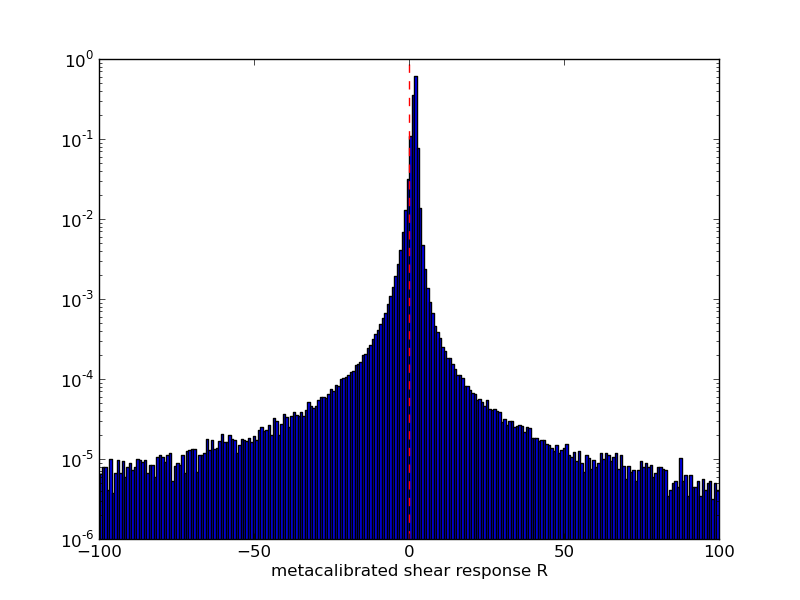
\includegraphics[width=0.45\textwidth]{./Plots/regauss-r-histogram.png}
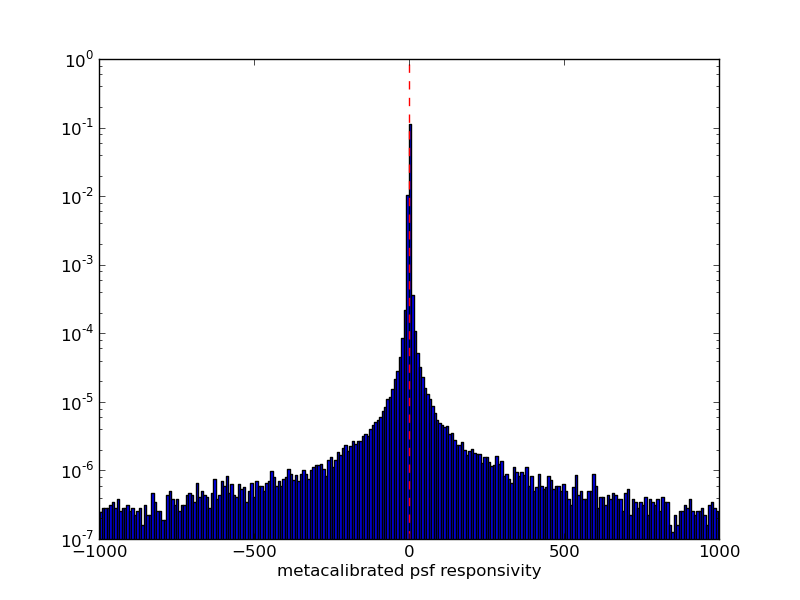
\includegraphics[width=0.45\textwidth]{./Plots/regauss-a-histogram.png}
\caption{{\bf Top:} Normalized distribution of meta-calibration shear responsivities from Regaussianization, on the Control-Ground-Constrant branch of the GREAT3 simulations.  {\bf Bottom:} Distribution of meta-calibration psf ellipticity responsivities from Regaussianization, on the Control-Ground-Constrant branch of the GREAT3 simulations. Vertical red dashed lines are drawn at zero for reference in both panels.}
\label{fig:calibhist}
\end{figure}


\begin{figure*}
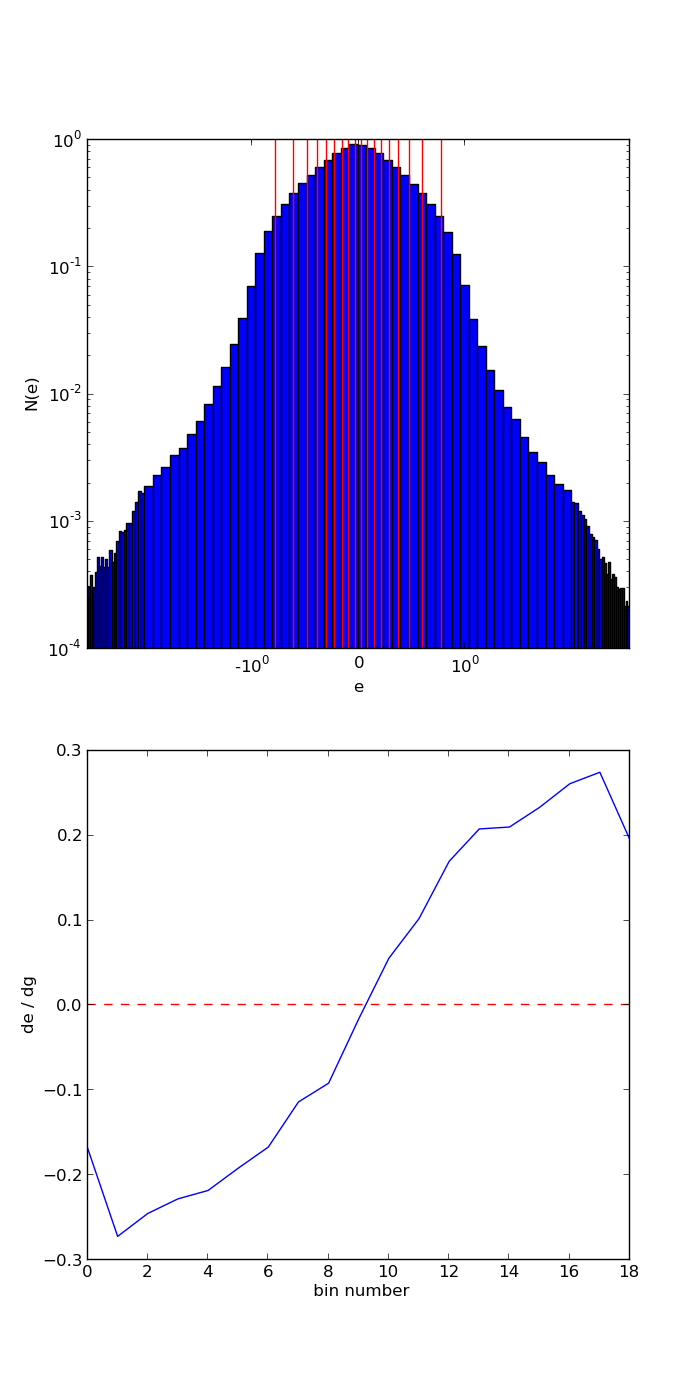
\includegraphics[width=0.3\textwidth]{./Plots/regauss-opt-shear_plots-prior_derivs.png}
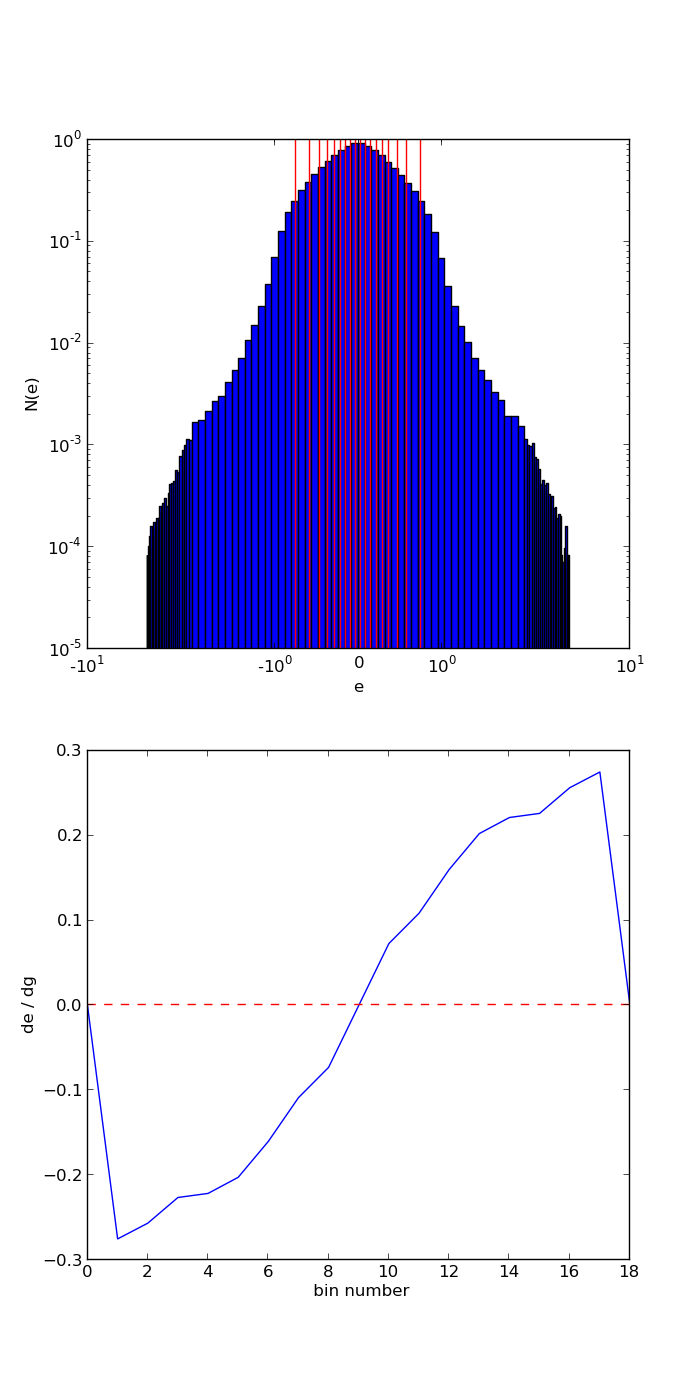
\includegraphics[width=0.3\textwidth]{./Plots/ksb-opt-shear_plots-prior_derivs.png}
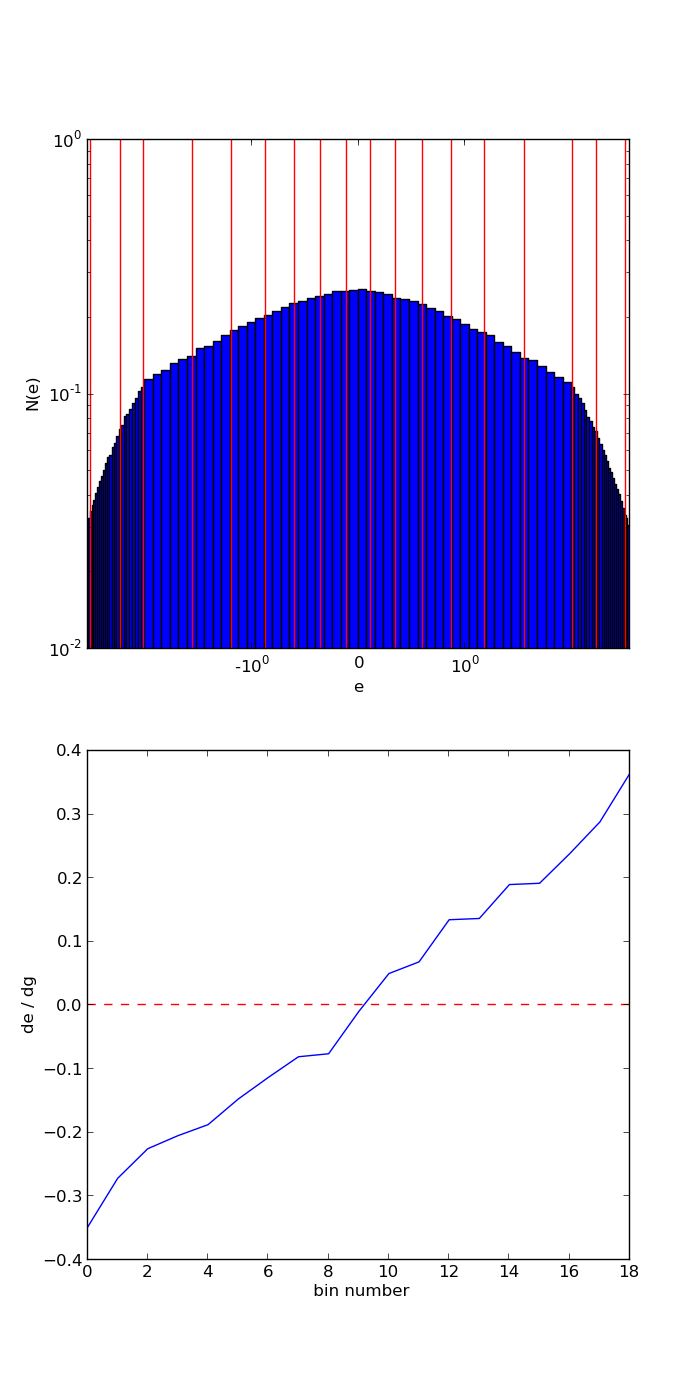
\includegraphics[width=0.3\textwidth]{./Plots/moments-opt-shear_plots-prior_derivs.png}
\caption{I do not like these figures. Treat them as placeholders for now.\\
Constructing the histogram estimator for the three shape measurement methods. {\bf Top} panels show measured shape distribution for each (from {\bf right} to {\bf left}) of the regauss, ksb, and moments methds. Vertical red lines show bin edges for a scheme with only 20 bins (much less than used in the estimation). {\bf Bottom} panels show the derivative $\frac{d\,p(e)}{d{e}}$ for each of the histograms. Abscissa are truncated at $\pm 4$, but the estimator runs over bins including all objects.
}
\label{fig:estimator}
\end{figure*}

If we have a poor model for the unlensed histogram, $h_{\rm fid}$, then the results will be biased. We can evaulate the distance from each field to the unlensed prior using equation~\ref{eqn:multnomial}, taking the probabilities $q_i$ from the unlensed prior and the histogram amplitudes from the current field, {after correcting for the estimated shear}. If the shear response measured for the unlensed prior is correct, then the performance of the estimator will depend only on the similarity of the prior to the measurement field. The likelihood can then be used as an objective criterion for the quality of the inference. 

\subsection{Relationship to previous implementations}

As shown in the GREAT3 results paper \citep{2015MNRAS.450.2963M}, an early version of
metacalibration was used in the GREAT3 challenge.  That implementation differs from the one
presented here and released publicly in association with this paper in two important ways: the model
for systematics was simpler than the one presented below (in particular, it neglected additive
systematics entirely) and the method for inferring shears from an ensemble of objects was entirely
different.  These differences are of sufficient importance that the GREAT3 results (especially the
ones for additive systematics) are not relevant to the implementation described here.


\section{Testing Framework}

\subsection{Estimation Algorithms}

Since the metacalibration method can in principle be used to calibrate shears from any per-object
shear algorithm, we chose three easily available shear estimation methods, all of which are
implemented in GalSim.  Two of these methods are more traditional shear estimation methods that have
somewhat different assumptions but are both based on object moments.  One method is not a standard
shear estimation method at all: we use linear combinations of the directly observed second moments
without correcting for the PSF at all.  In principle, the information about how those respond to
shear should be determined by metacalibration to correctly infer the shear.  THe difference in this
case is that instead of providing a small correction to the outputs of a PSF correction method, we
rely on metacalibration to do the entirety of the PSF correction, which is a very stringent test.

\subsubsection{Regaussianization}

 Re-Gaussianization \citep{2003MNRAS.343..459H} is a PSF correction method based on the use of the
 moments of the image and of the PSF to correct for the effects of the PSF on the galaxy shapes. It
 includes corrections for the non-Gaussianity of the galaxy profile
 \citep{2002AJ....123..583B,2003MNRAS.343..459H} and of the PSF (to first order in the PSF
 non-Gaussianity). The performance of this algorithm has been extensively studied in real data and
 simulations
 \citep[e.g.,][]{2005MNRAS.361.1287M,2012MNRAS.420.1518M,2013MNRAS.432.1544M,2015MNRAS.450.2963M}.

The outputs of the re-Gaussianization algorithm are PSF-corrected ``distortions'', which for an
object with purely elliptical isophotes with minor-to-major axis ratio $q$ and position angle
$\theta$ with respect to the $x$ axis in pixel coordinates would be defined as
\begin{equation}
(e_1, e_2) = \frac{1-q^2}{1+q^2}\left(\cos{2\theta},\sin{2\theta}\right).
\end{equation}
As discussed in \cite{2002AJ....123..583B}, the response of a distribution of galaxies with some intrinsic
distribution of distortions $p(e)$ to a shear is nonlinear in a way that depends on the $p(e)$
itself.  Conceptually, we can think of an ensemble shear estimator using re-Gaussianization outputs
as
\begin{equation}
\hat{\gamma}_j = \frac{\langle e_j\rangle}{\mathrm{d}\langle e_j\rangle/\mathrm{d}\gamma_j}
\end{equation}
where the denominator gives the response of the ensemble average distortion to a shear (often called
the responsivity).  Estimators of this shear responsivity use the observed galaxy $p(e)$ and its
moments, and for typical $p(e)$, the denominator is around $1.7$--$1.8$.

\subsubsection{KSB}

The KSB method \citep{1995ApJ...449..460K} parametrises galaxies and stars according to their
weighted quadrupole moments.  The main assumption of the KSB method is that the PSF 
can be described as a small but highly anisotropic distortion
convolved with a large circularly symmetric function. 
With that assumption, the shear can be recovered to
first-order from the observed ellipticity of each galaxy via
\begin{equation} \label{eqn:weight}
\gamma=P_{\gamma}^{-1}\left(e^{\rm obs}-\frac{P^{\rm sm}}{P^{\rm sm*}}e^{*}\right),
\end{equation}
where asterisks indicate quantities that should be measured from the
PSF model at that galaxy position, $P^{\rm sm}$ is the
smear polarisability (see \citealt{2006MNRAS.368.1323H} for definitions) 
and $P_\gamma$ is the correction to the shear
polarisability that includes the smearing with the isotropic component
of the PSF. The ellipticities are constructed from 
weighted quadrupole moments, and the other quantities involve
higher order moments. A  circular Gaussian weight 
of scale length $r_g$ is used, where $r_g$ is galaxy
size.

The KSB method returns a per-object estimate of the shears $(\hat{\gamma}_1, \hat{\gamma}_2)$. We can use
metacalibration to infer the shear while removing multiplicative and additive biases in the method.

\subsubsection{Linear Moments}

As mentioned previously, the third method we use does not involve PSF-corrected galaxy shapes.
Instead, we use linear combinations of the second moments of galaxy images.  The motivation behind
this choice is as follows.  One way to estimate the distortion $(e_1,e_2)$ is via combinations of
the second moments of the light profile,
\begin{equation}
\langle x_i\rangle = \frac{\int x_i w({\mathbf x}) I({\mathbf x}) \mathrm{d}^2{\mathbf x}}{\int w({\mathbf x}) I({\mathbf x}) \mathrm{d}^2{\mathbf x}}
\end{equation}
for $i=1, 2$,
\begin{equation}
M_{ij} = \frac{\int (x_i-\langle x_i\rangle)(x_j-\langle x_j\rangle) w({\mathbf x}) I({\mathbf x}) \mathrm{d}^2{\mathbf x}}{\int w({\mathbf x}) I({\mathbf x}) \mathrm{d}^2{\mathbf x}}
\end{equation}
for $i,j=1,2$, and finally 
\begin{equation}\label{eq:moments-div}
e_1 = \frac{M_{11}-M_{22}}{M_{11}+M_{22}}, \qquad e_2 \frac{2M_{12}}{M_{11}+M_{22}}.
\end{equation}

One source of noise in traditional moments based methods is the division of two noisy quantities in
Eq.~\ref{eq:moments-div}, typically followed by further division by other noisy quantities to remove
the dilution of the galaxy shape by the PSF.  Thus, as a final example of a statistic that we will
attempt to use as a calibrated shear estimator with metacalibration, we define the following linear
combinations of moments:
\begin{equation}
\hat{M}_i = (M_{11}-M_{22}, 2M_{12}).
\end{equation}

Clearly these moments include a number of nuisance quantities, like the galaxy flux and size.  They
also do not include any PSF correction whatsoever.  In principle, metacalibration should be able to
nonetheless determine the response of this statistic to shear,
$\mathrm{d}\hat{M}_i/\mathrm{d}\gamma$, and produce a reliable shear estimate, provided that the
model for the predominant sources of systematics follows that in Eq.~\ref{eqn:edist_model}.  This is
a quite stringent test of the metacalibration method.

\subsection{Simulated Images}

We use the GREAT3 simulation framework as the source of simulated images that we use for testing
purposes.  For more detail about that simulation framework, see the GREAT3 handbook
\citep{2014ApJS..212....5M} and results paper \citep{2015MNRAS.450.2963M}, or the publicly
available software\footnote{\url{https://github.com/barnabytprowe/great3-public}}.

In brief, we use simulated ``branches'' containing 200 ``subfields''.  Each subfield contains $10^4$
galaxies placed on a $100\times 100$ grid; the galaxies in a given subfield all have the same
(unknown) shear and the same known PSF.  The galaxy population within a subfield follows a
distribution of signal-to-noise ratio, size, ellipticity, and morphology based on that in the {\it
  Hubble Space Telescope} ({\it HST}) COSMOS survey
\citep{2007ApJS..172..196K,2007ApJS..172....1S,2007ApJS..172...38S}, roughly approximating a galaxy
sample with a depth of $I<25$.  To ensure that most methods will be able to measure all galaxies, an
effective signal-to-noise cut of $\gtrsim 12$ and a minimal resolution cut was imposed (resulting in
different sets of galaxies in subfields that have different-sized PSFs).  90$^\circ$ rotated pairs
of galaxies were included, to cancel out shape noise \citep{2007MNRAS.376...13M}.  The PSF in the
simulations comes from the combination of an optics model from a ground-based telescope, along with
a Kolmogorov PSF with a typical ellipticity variance.  Thus, the galaxy and PSF properties are
non-trivially complicated.  The noise is stationary Gaussian noise.  The
ultimate goal is to estimate the average shear in each subfield in an unbiased way, without any
multiplicative bias or correlations with the per-subfield PSF ellipticity.

One important distinction between GREAT3 and the real Universe that we will have to consider is the
mean shear.  In a real patch of sky comparable to the size of a large survey, the expected mean
shear is zero.  In GREAT3, while lensing shears $g_1$ and $g_2$ are drawn from a distribution with
zero mean, the fact that there are only 200 subfields means that effectively only 200 draws from
that distribution were made, and that is not enough to have an effective mean shear of zero.  Thus,
for all of the results below, we will take the averages of the true shears per component as a known
quantity instead of doing a fully blind analysis, since the deviation of those quantities from zero
is just due to the artificial nature of the simulation design.

We consider two sets of galaxy populations.  One comes directly from {\it HST} images, and includes
a process to remove the HST PSF before shearing (both operations being carried out in Fourier space)
and convolving with the final target PSF \citep{2012MNRAS.420.1518M}.  The other galaxy population
consists of simple parametric representations of those {\it HST} images.  These populations have the
same effective distributions of size, ellipticity, and so on, but one includes realistic galaxy
morphology while the other only includes such realism as can be captured by the sum of two
S\'{e}rsic profiles.  In the language of GREAT3, we use simulations corresponding to
control-ground-constant (describing the parametric galaxy sample, ground-based simulated data, with
a constant per-subfield shear) and real$\_$galaxy-ground-constant (the realistic galaxy sample),
denoted CGC and RGC.


\subsubsection{Control Ground Constant without Aberrations}

Before analyzing the GREAT3 results, we analyze a newly-generated set of simulations that is closely
analogous to the GREAT3 CGC branch (parametric galaxy profiles), but with one modification to avoid
a problem raised in the results paper \citep{2015MNRAS.450.2963M}.  There, it was noted that the CGC
branch has a number of outlier fields related to unusually large optical PSF aberrations,
specifically defocus and trefoil.  Thus, our first simulated dataset is designed exactly like CGC
but with all aberrations in the optical PSF set to zero, to ensure reasonable consistency of data
quality.  Note that the atmospheric PSF is still drawn from a distribution of seeing values for each
subfield.

\towriteemh{Performance expectations on this branch.}
\towriteemh{Briefly summarize calibration results for this branch.}


\subsubsection{Real Ground Constant without Aberrations}

The next branch we analyze is similar to the previous one, but with realistic galaxies.  Thus, we
refer to this branch as ``RGC without aberrations''.

\towriteemh{Performance expectations on this branch.}
\towriteemh{Briefly summarize calibration results for this branch.}


\subsubsection{Control Ground Constant}

After testing metacalibration on the simulations without aberrations, we now turn to the actual
GREAT3 simulated data in the CGC branch, including parametric galaxies.

\towriteemh{Performance expectations on this branch.}
\towriteemh{Briefly summarize calibration results for this branch.}

\subsubsection{Real Ground Constant}

Next, we analyze the actual GREAT3 simulations in the RGC branch, with realistic galaxy morphology.

\towriteemh{Performance expectations on this branch.}
\towriteemh{Briefly summarize calibration results for this branch.}
\todoemh{Generate ksb metacalibration catalogs for this branch. }
\todoemh{Generate moments metacalibration catalogs for this branch.}
\toplotemh{Plot ksb results for this branch.}
\toplotemh{Plot moment results for this branch.}

\subsubsection{Real Ground Constant with constant aberrations}

One issue of concern is how to understand outlier fields.  In GREAT3, there was a concern that some
outliers were due to failure of our model for interpreting the per-object shapes in fields that had
large aberrations. {\it Eric, should I add a plot showing why we came to these conclusions, i.e.,
  the distributions of defocus and so on for outliers?  Or just paraphrase its conclusions?}  As a
way to understand this, we generated a version of RGC that had quite large aberrations that were
identical in each field: specifically defocus of $0.5$ waves and one component of trefoil of $0.1$
wave.

\towriteemh{Performance expectations on this branch.}
\towriteemh{Briefly summarize calibration results for this branch.}
\toplotemh{Plot regauss results for this branch.}
\toplotemh{Plot ksb results for this branch.}
\toplotemh{Plot moment results for this branch.}





\begin{figure*}
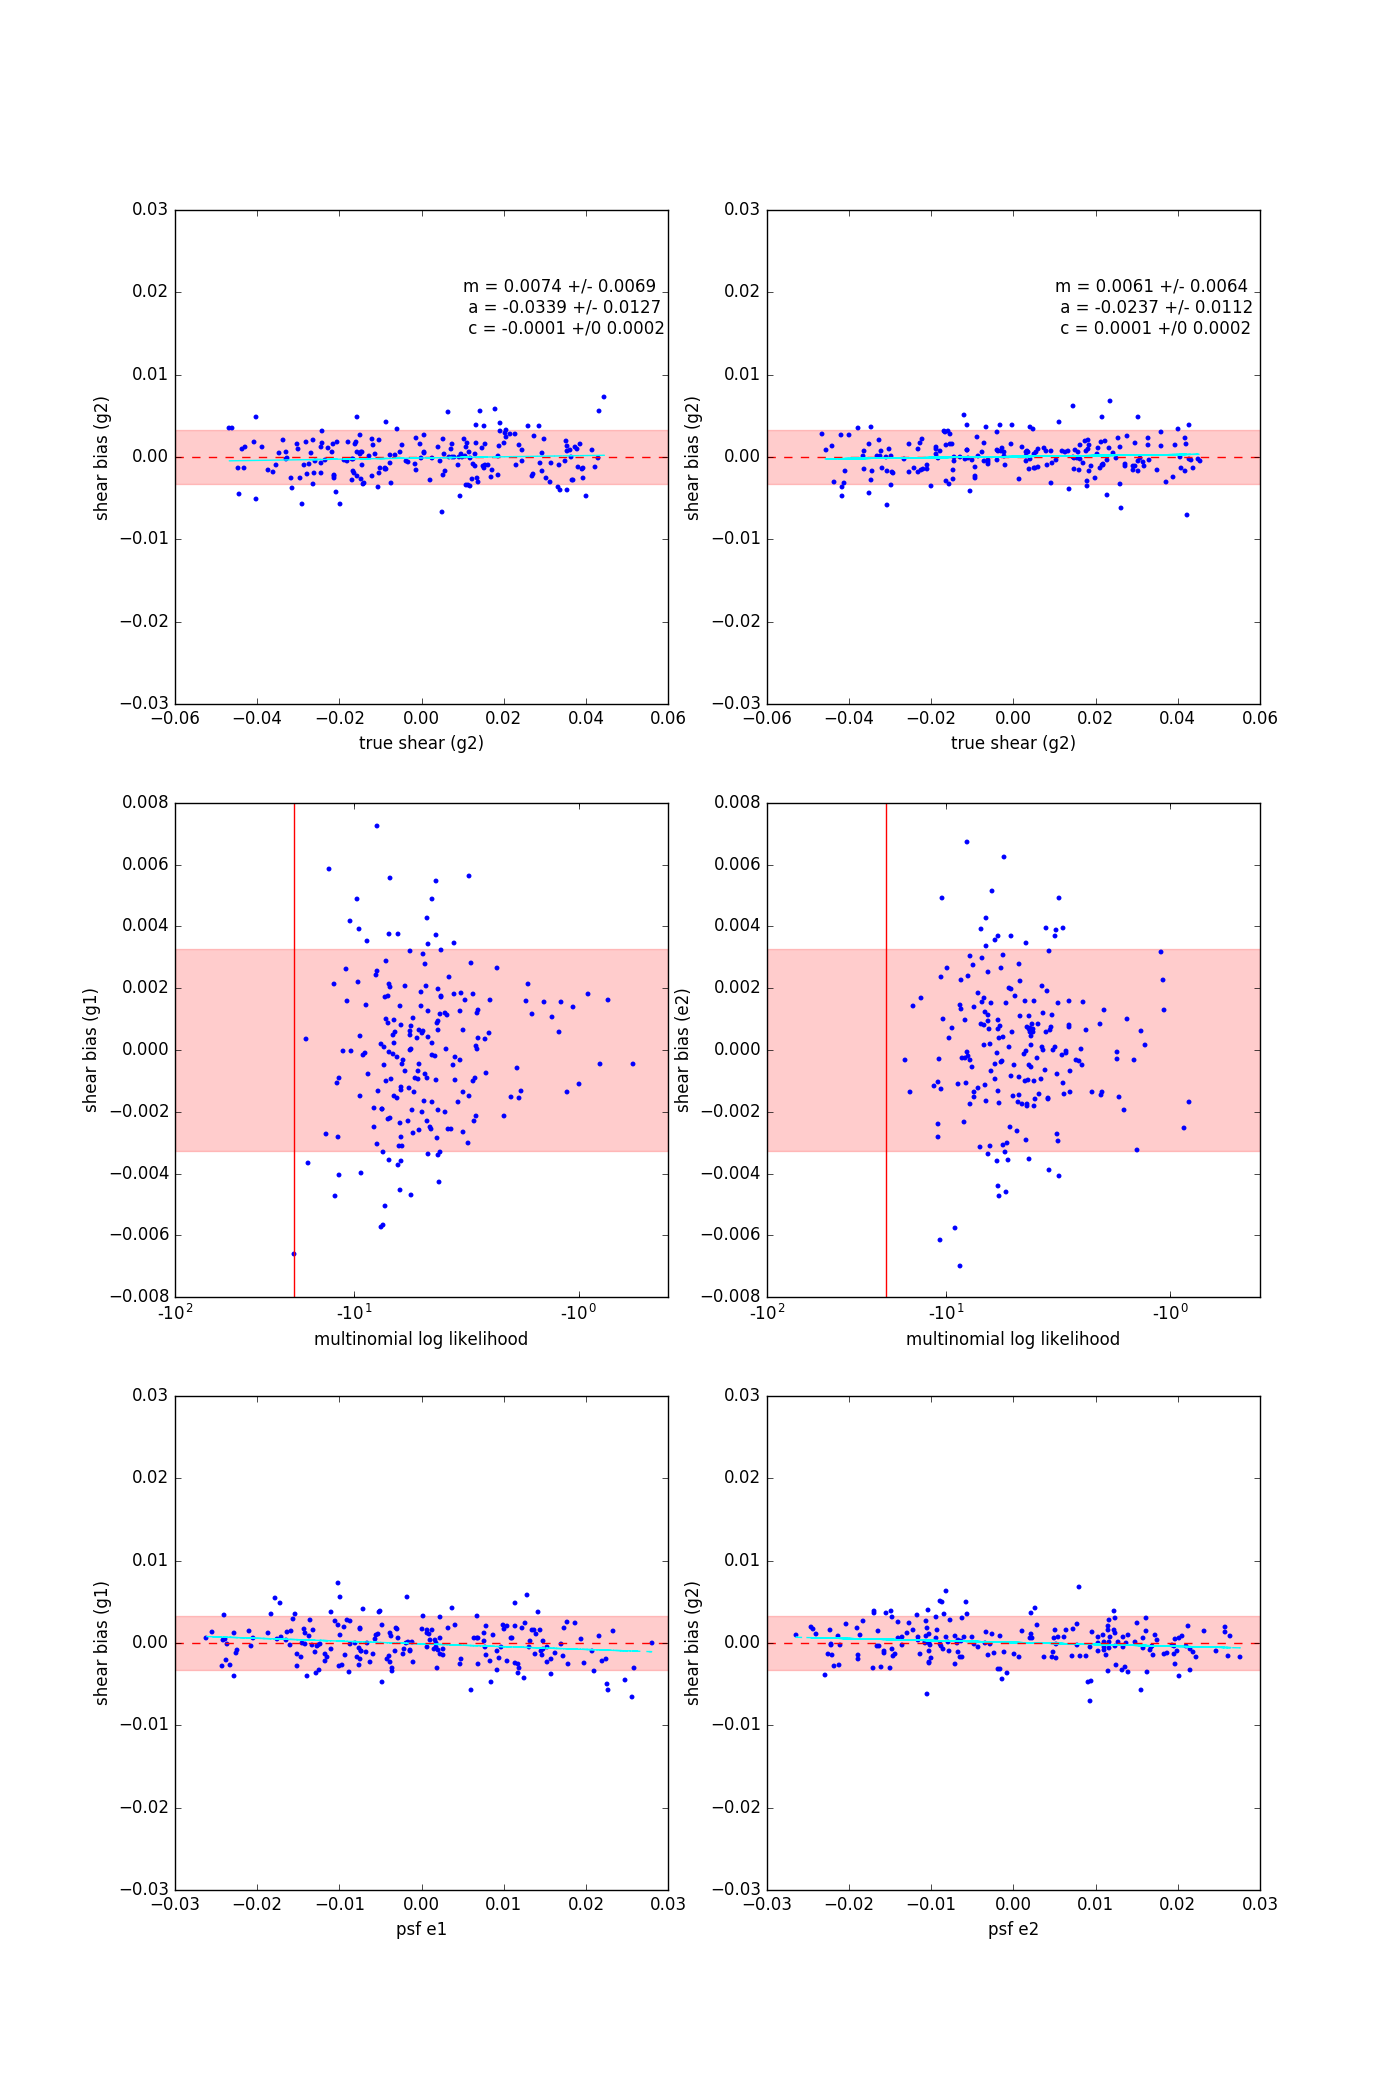
\includegraphics[width=0.31\linewidth]{./Plots/noaber-regauss-opt-shear_plots.png}
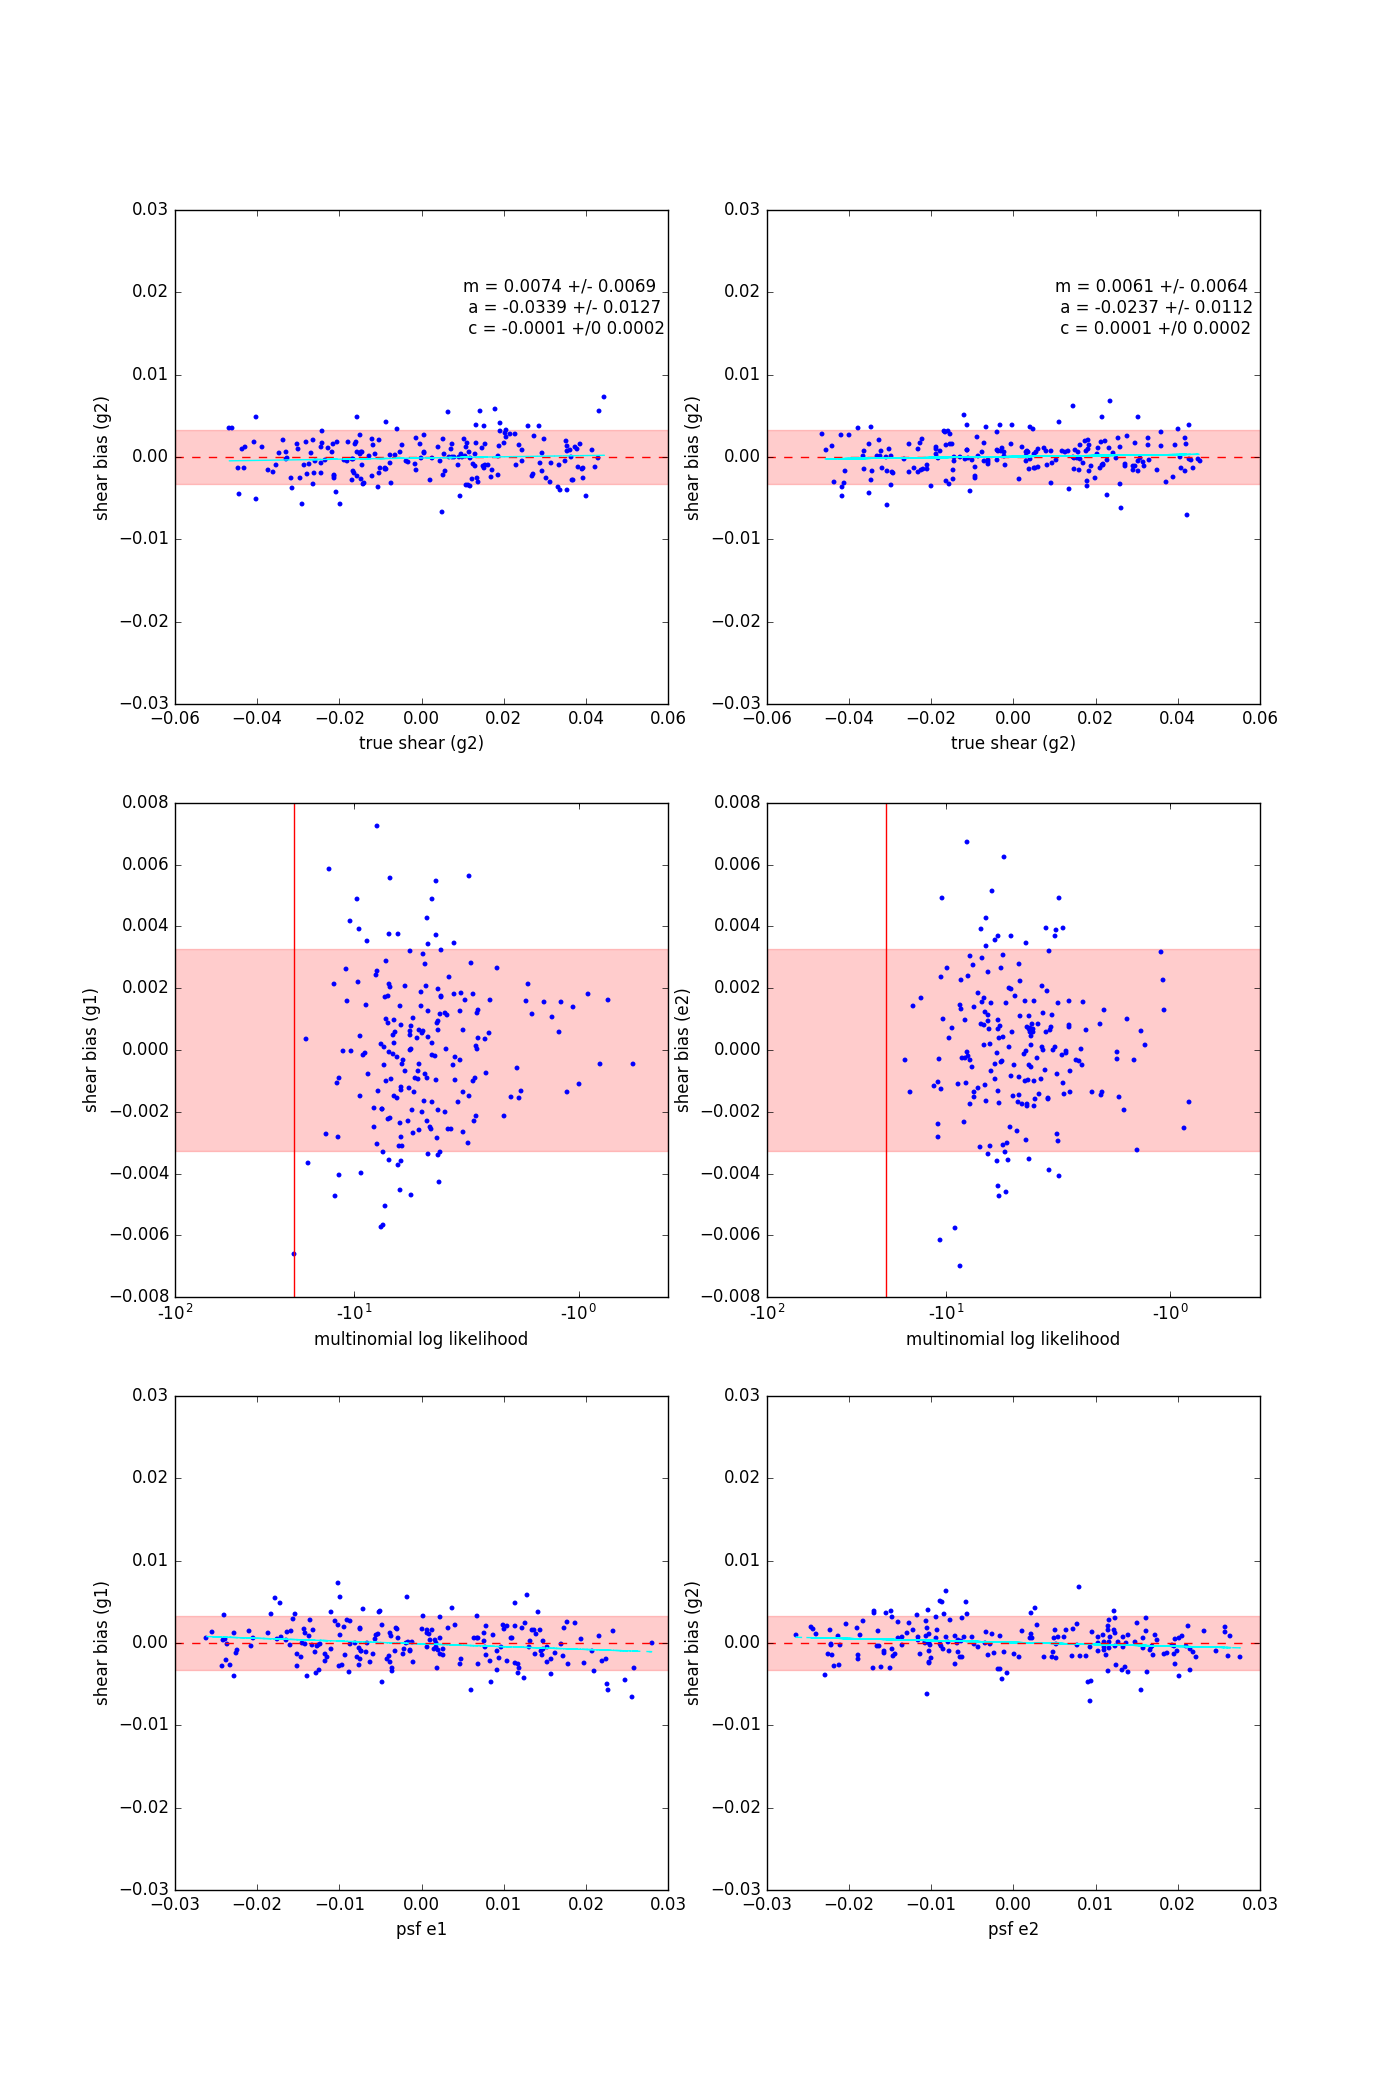
\includegraphics[width=0.31\linewidth]{./Plots/noaber-regauss-opt-shear_plots.png}
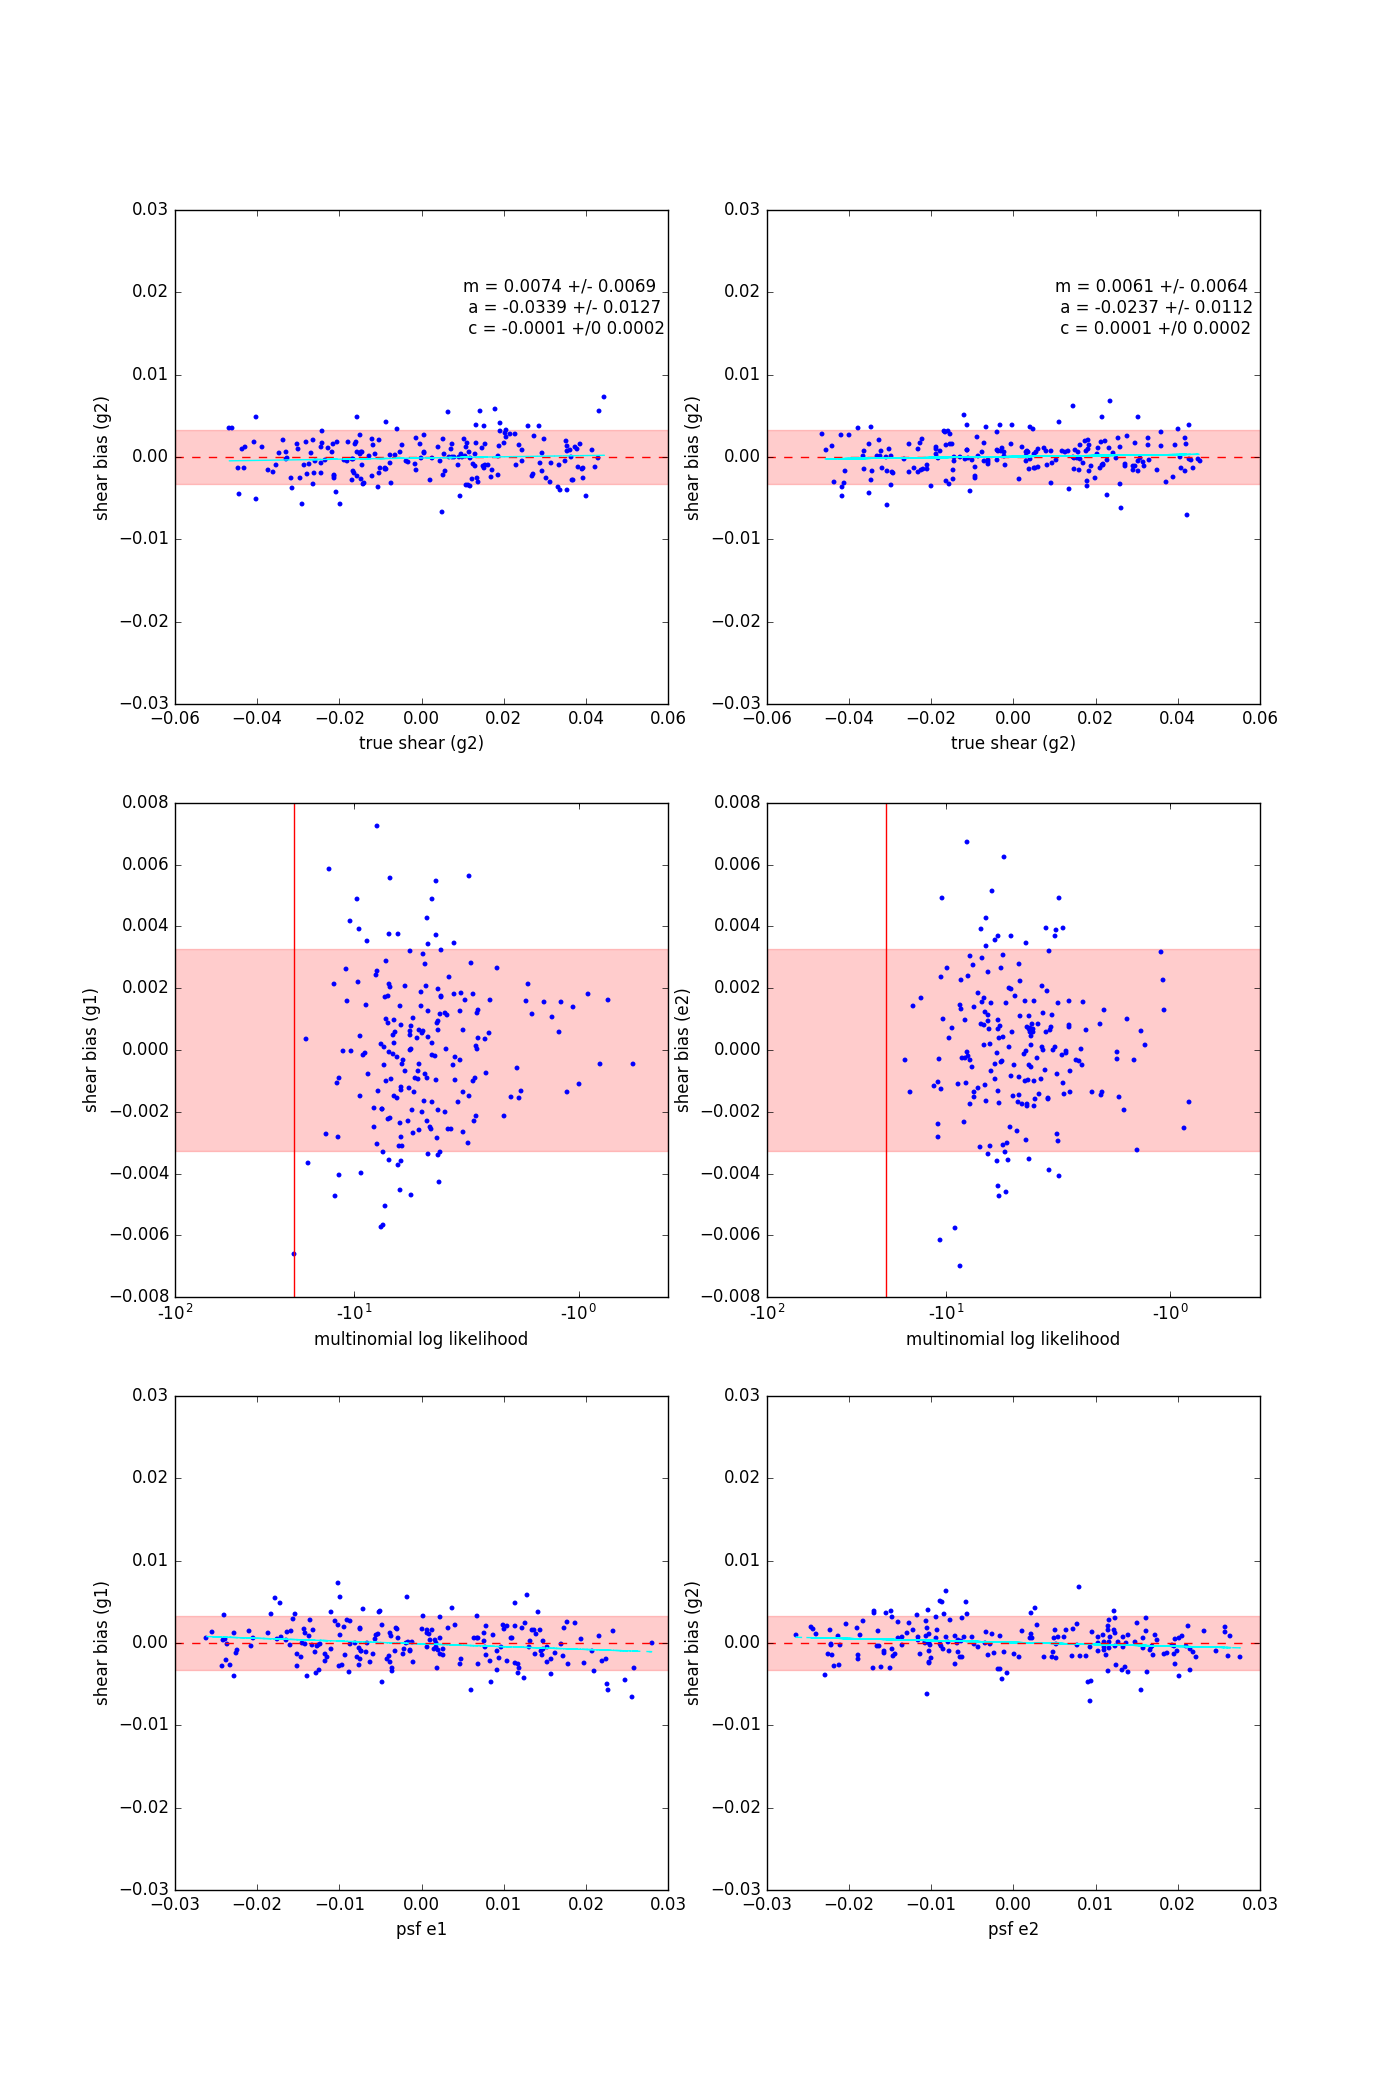
\includegraphics[width=0.31\linewidth]{./Plots/noaber-regauss-opt-shear_plots.png}
\caption{Results of metacalibration for regauss on CGC-no aberrations}
\end{figure*}


\begin{figure*}
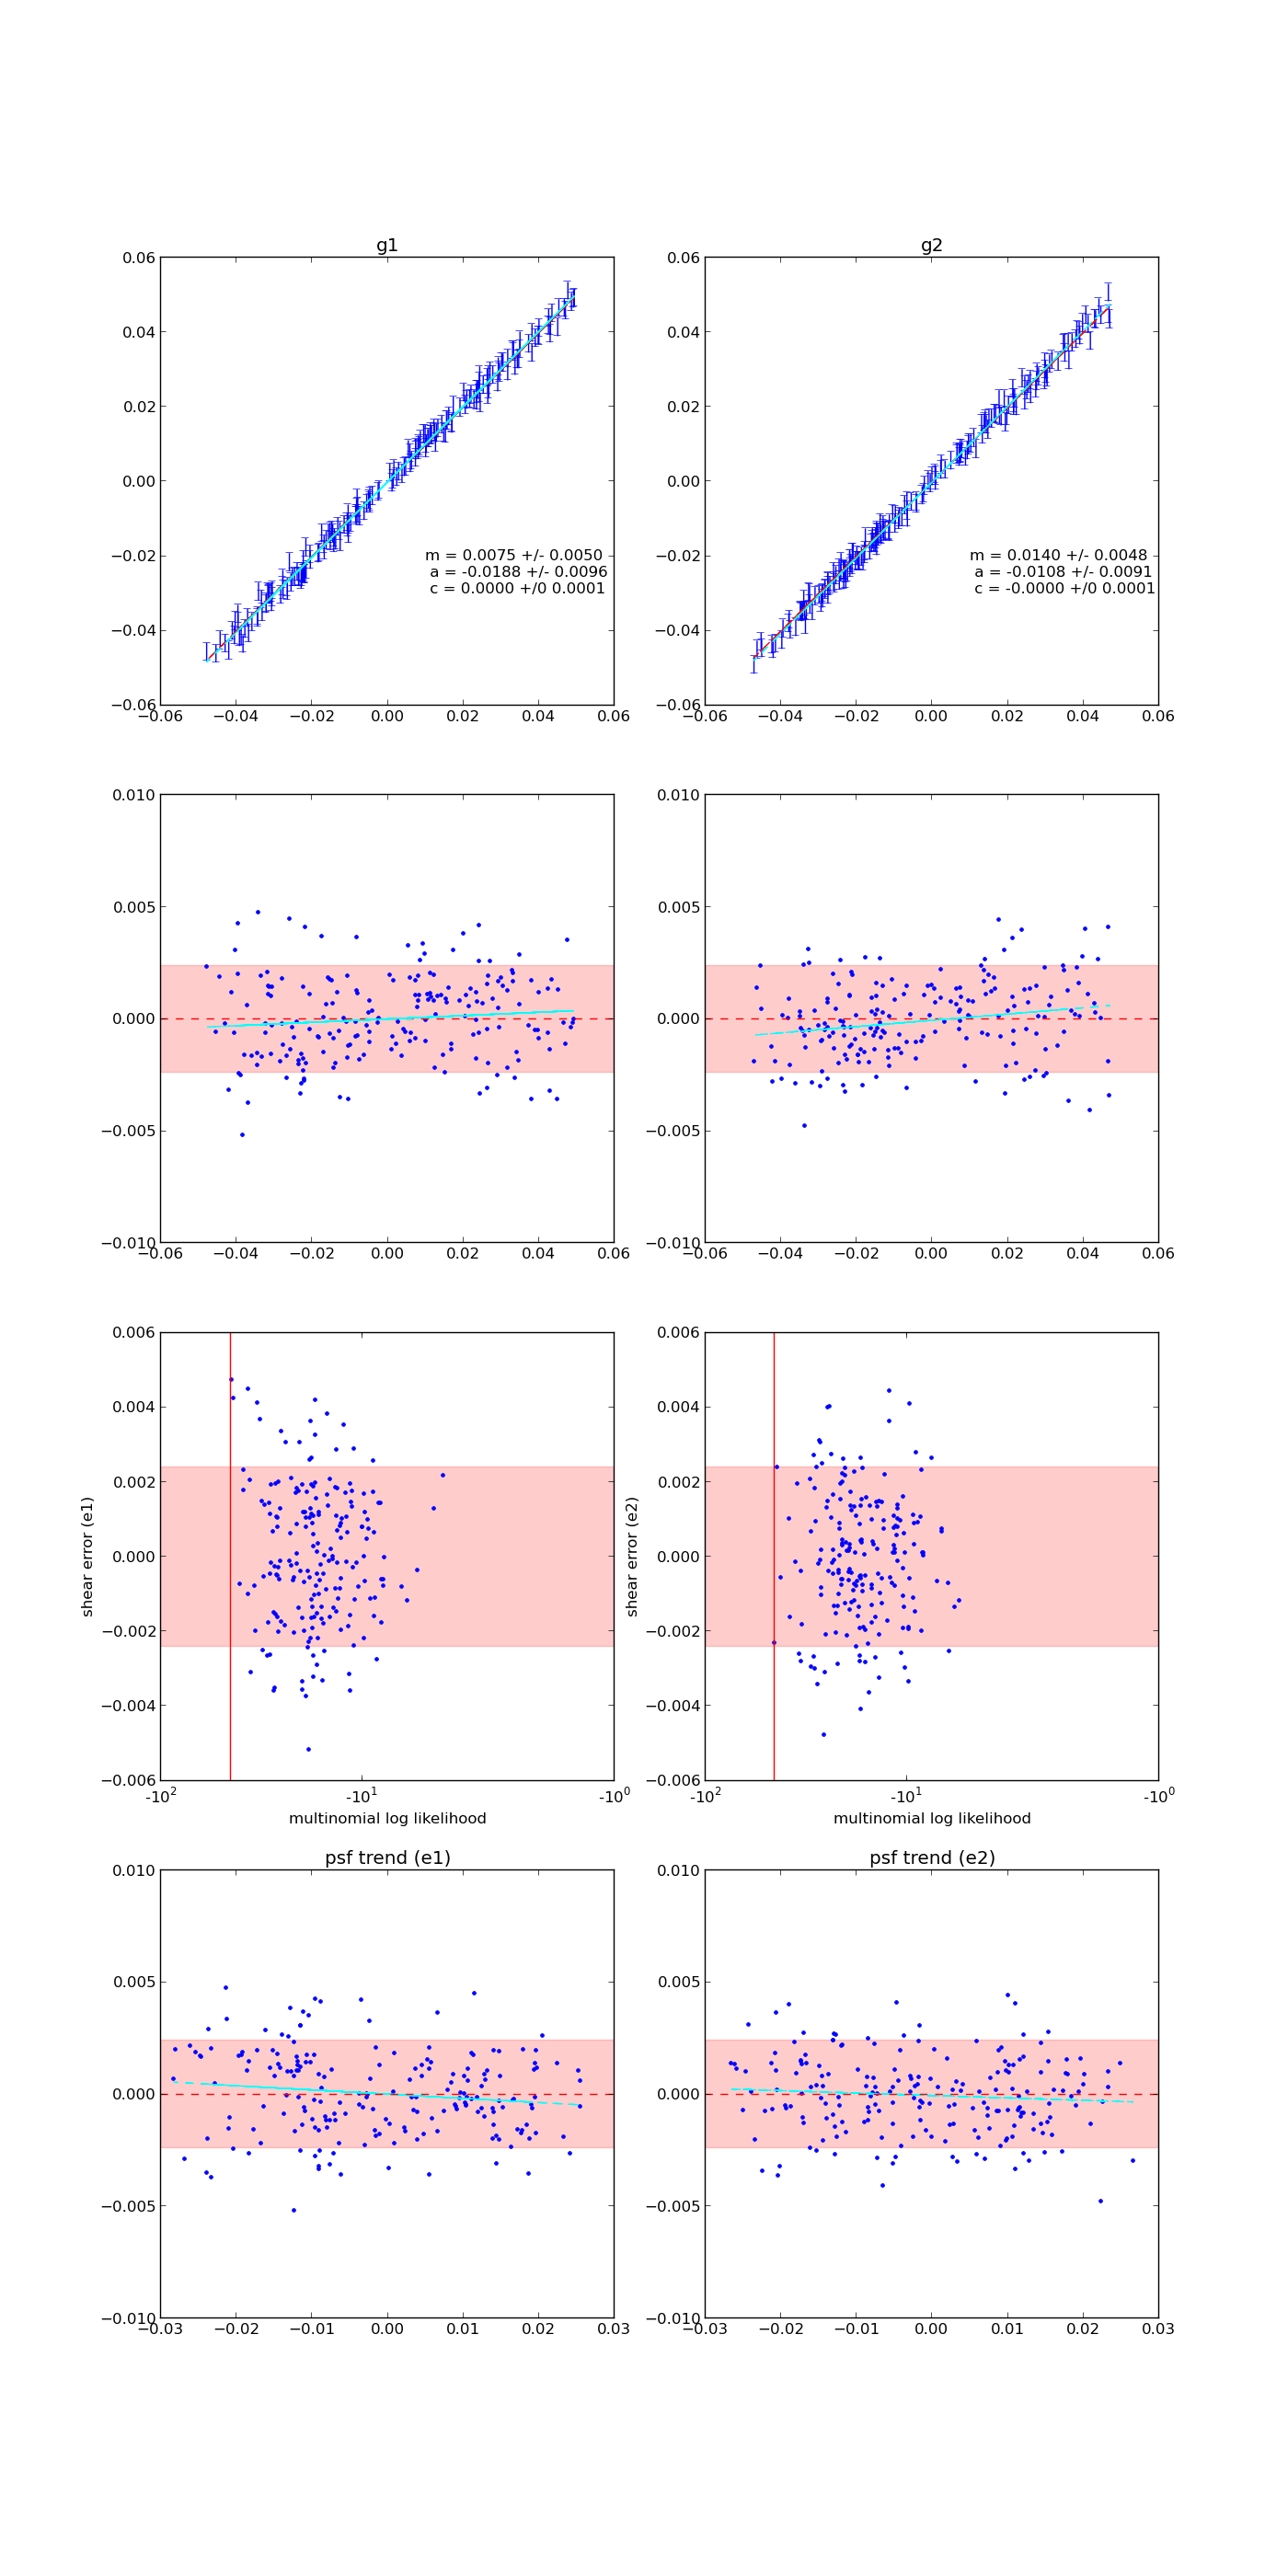
\includegraphics[width=0.31\linewidth]{./Plots/rgc-noaber-regauss-opt-shear_plots.png}
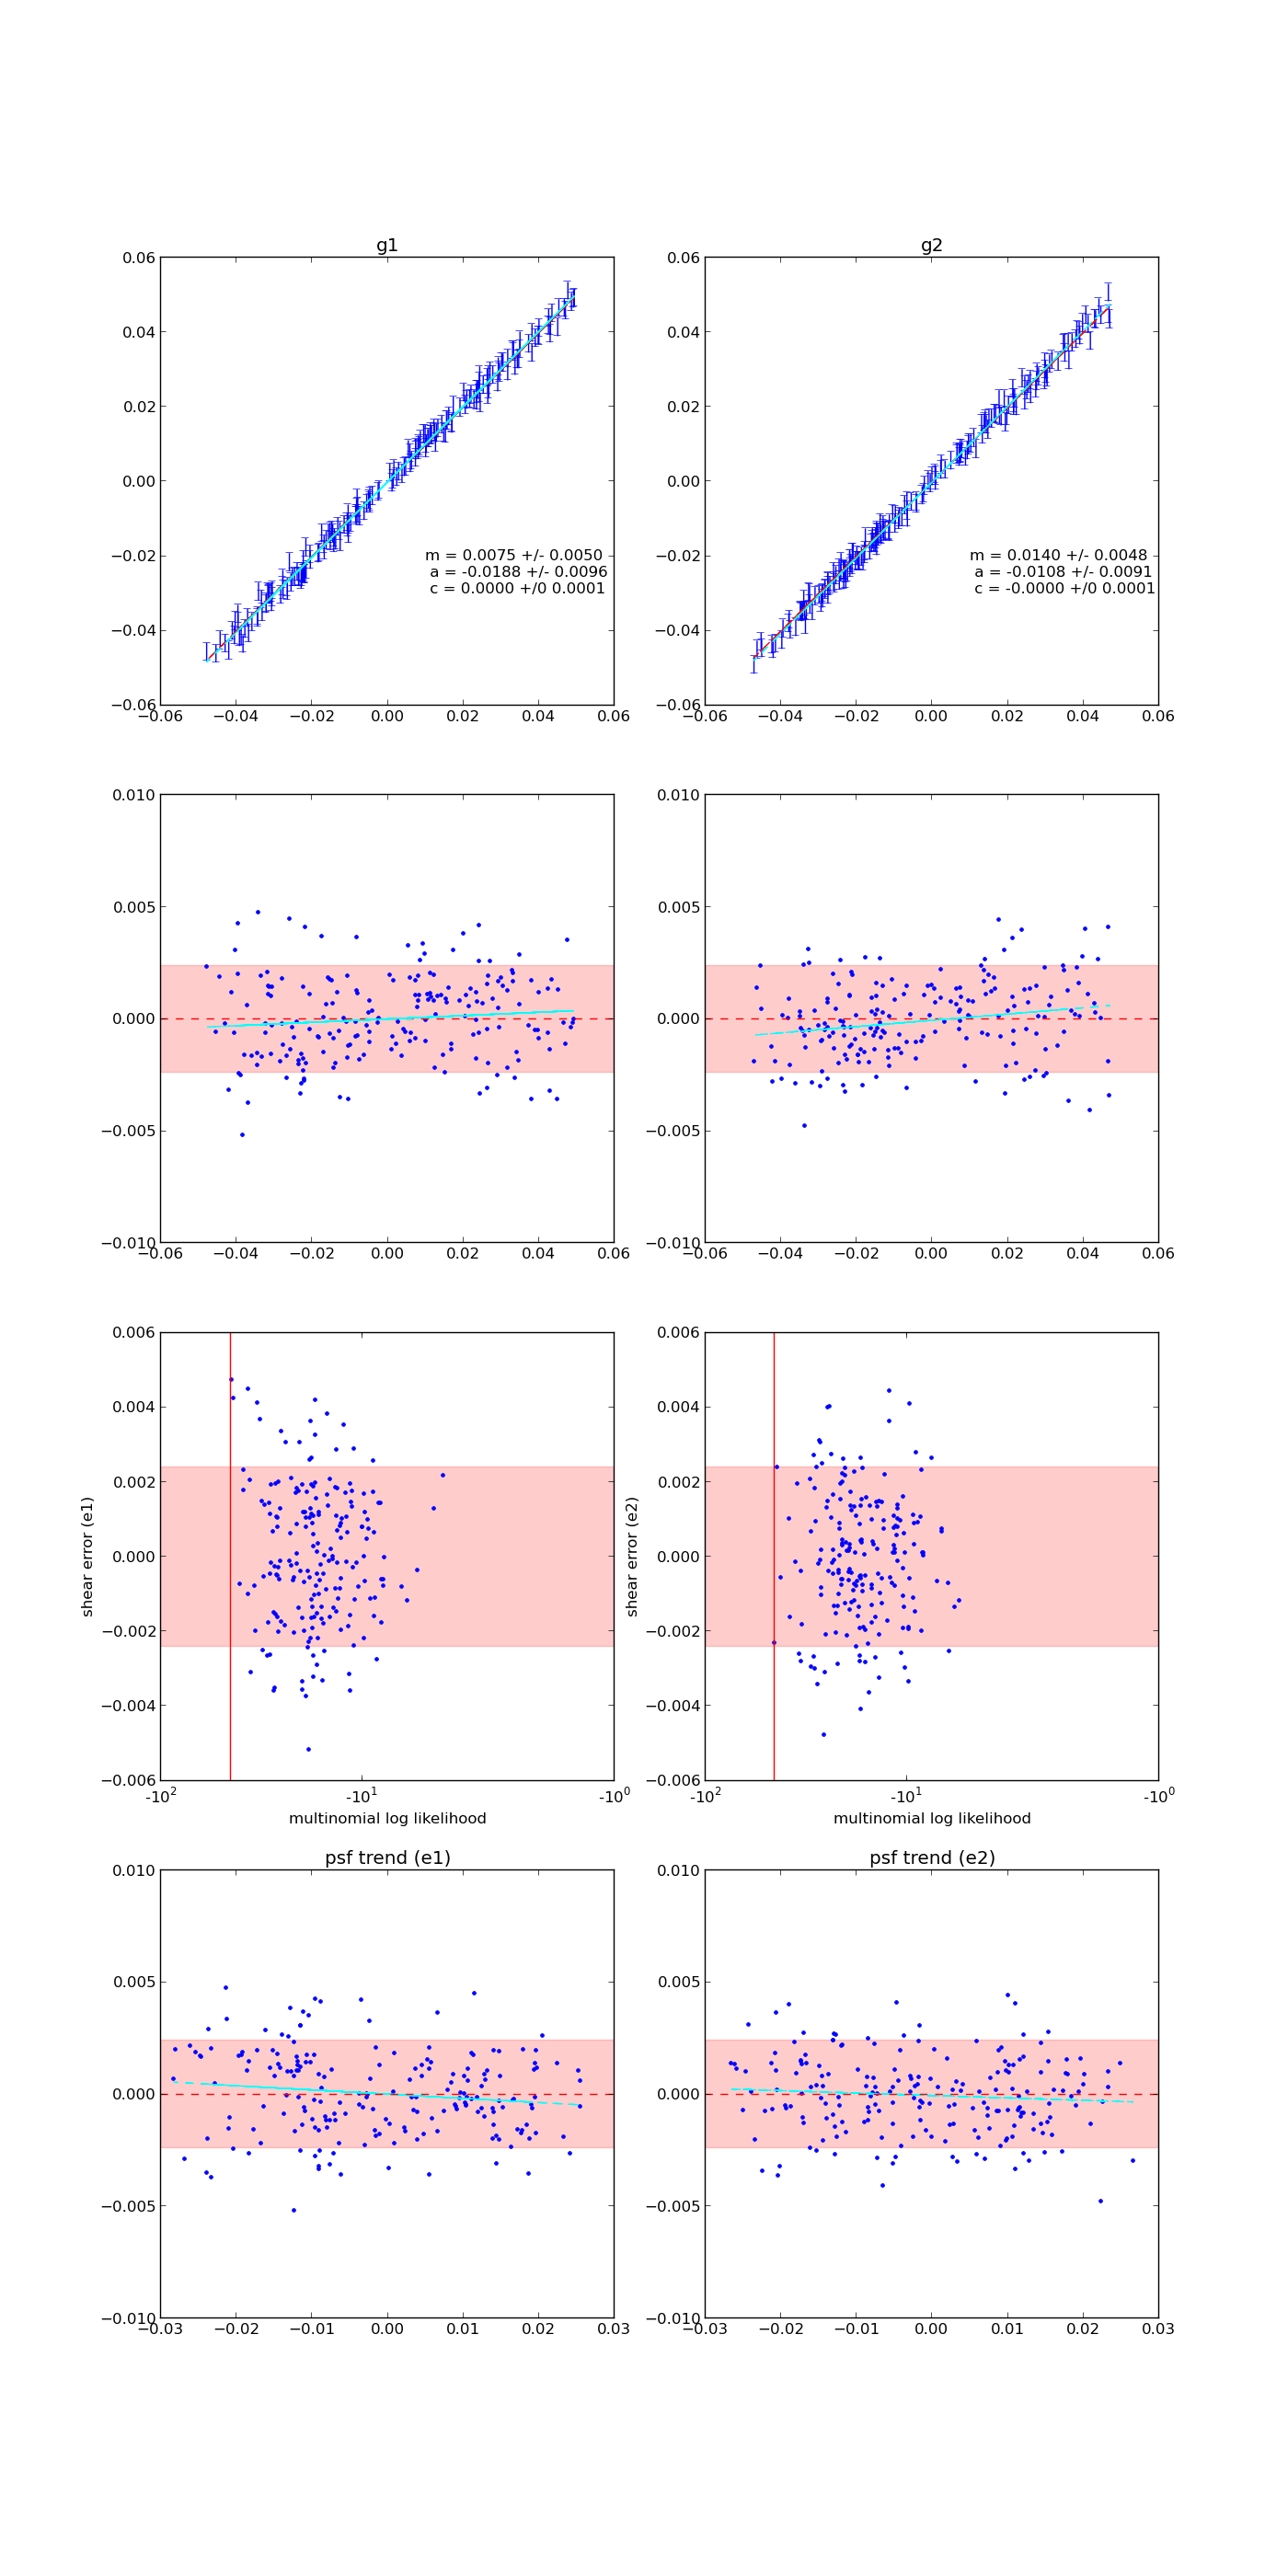
\includegraphics[width=0.31\linewidth]{./Plots/rgc-noaber-regauss-opt-shear_plots.png}
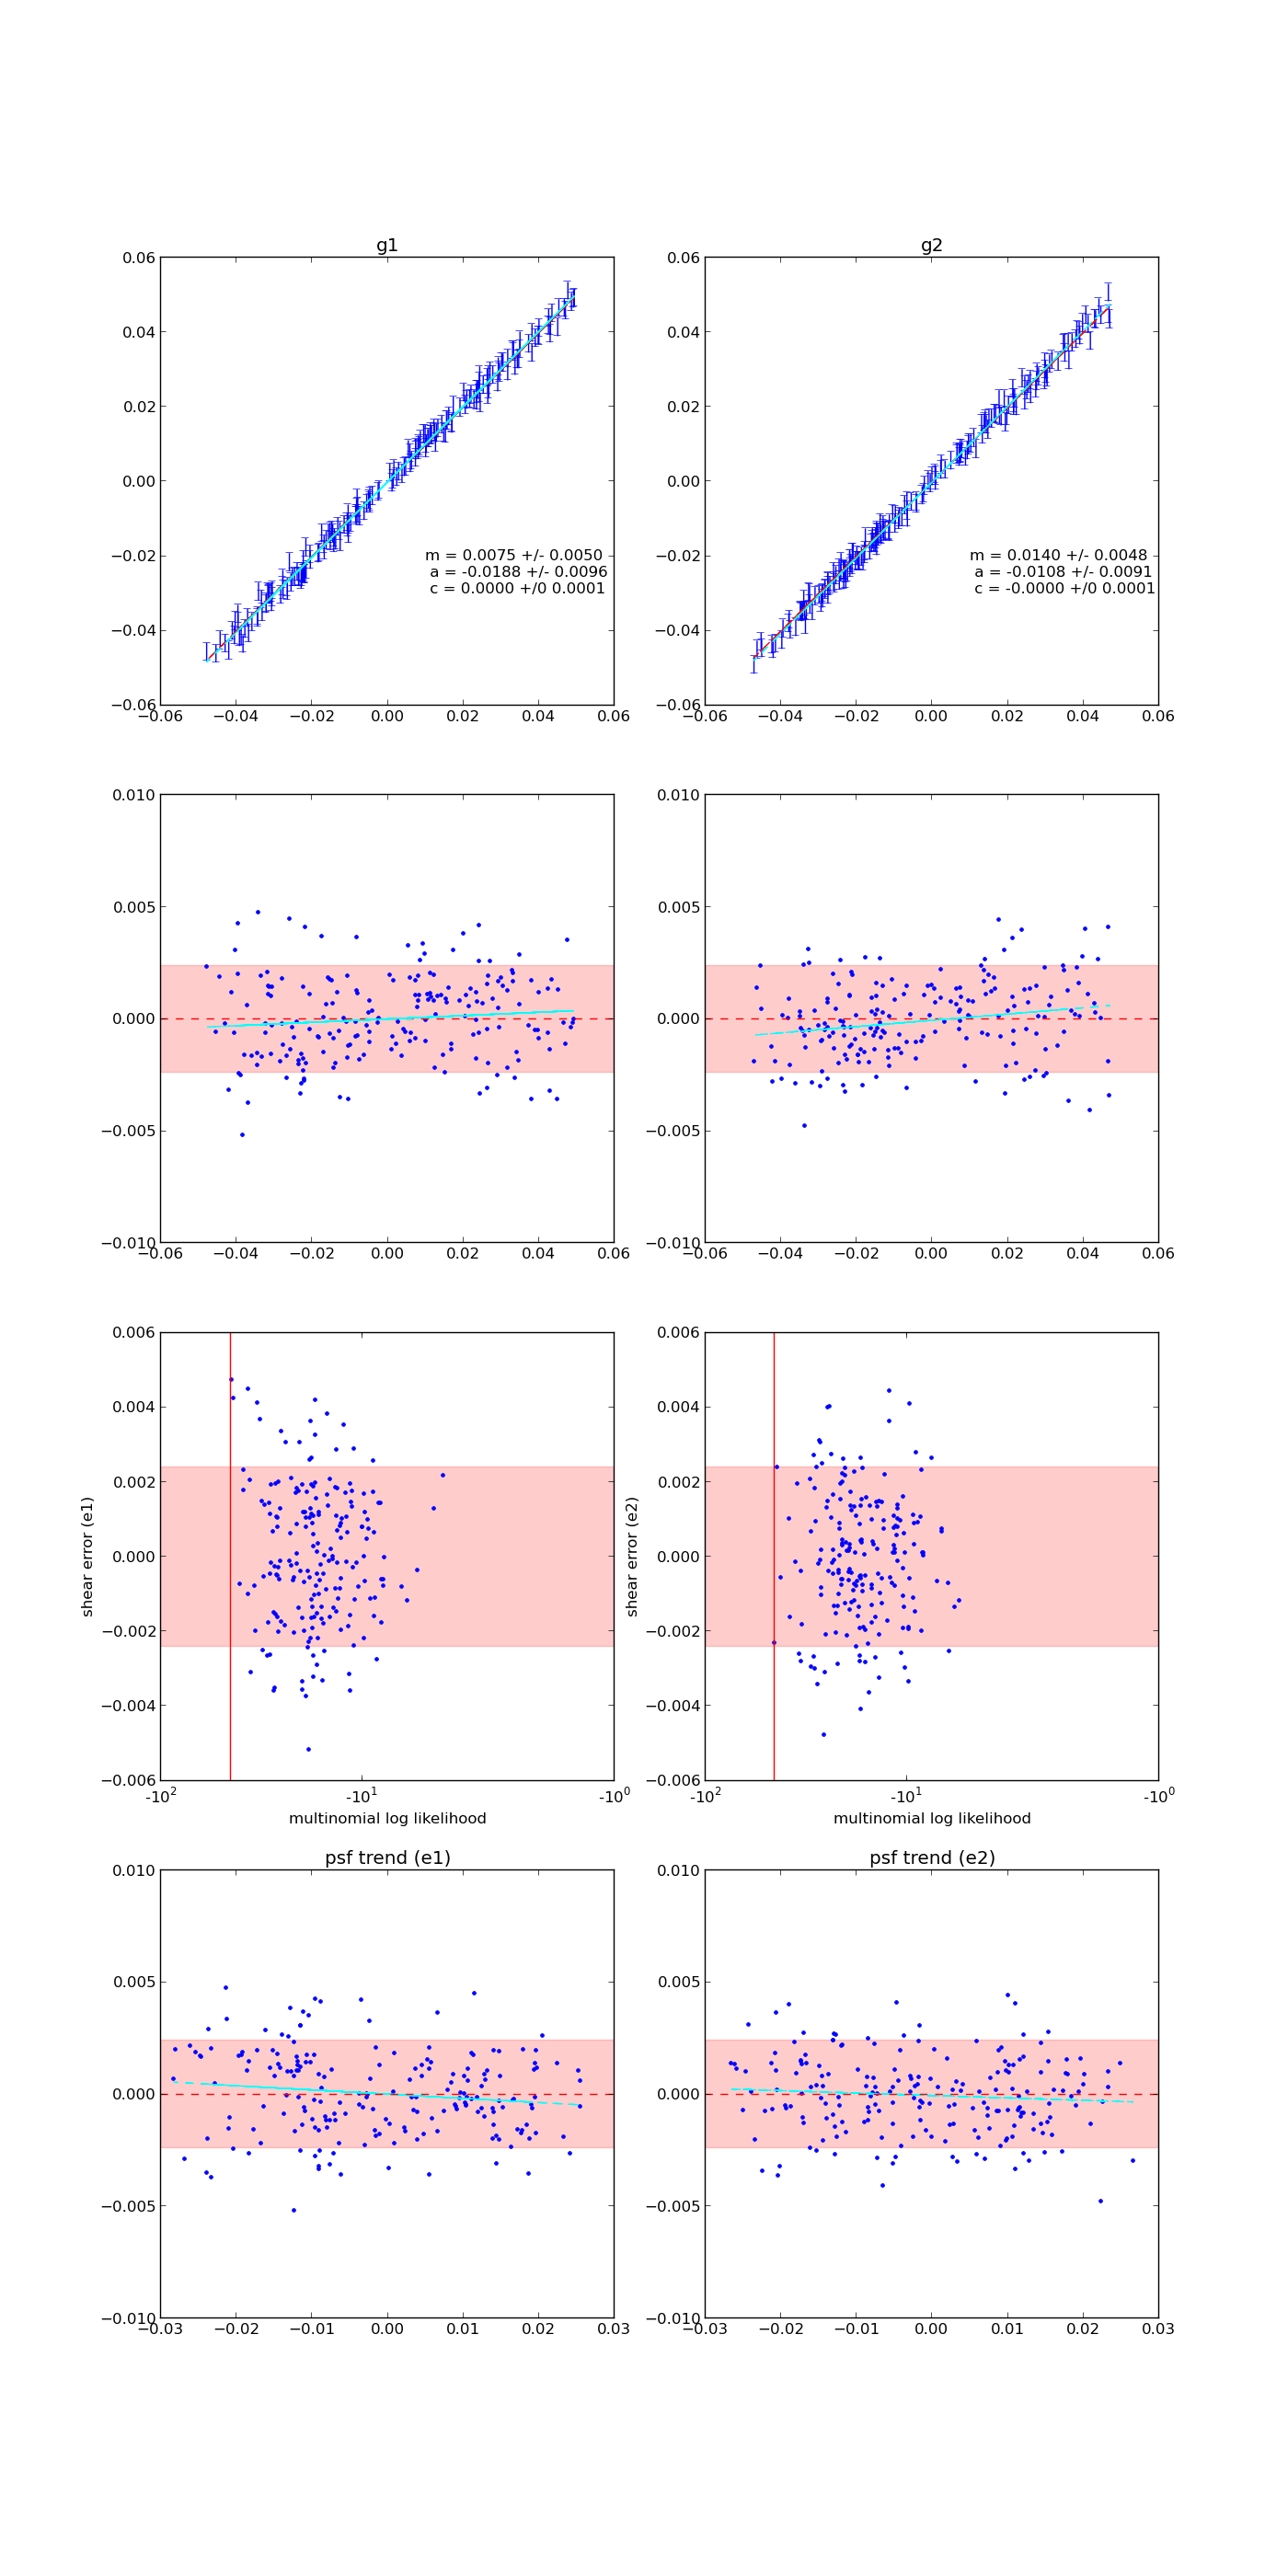
\includegraphics[width=0.31\linewidth]{./Plots/rgc-noaber-regauss-opt-shear_plots.png}
\caption{Results of metacalibration for regauss on CGC with no aberrations. From {\bf right} to {\bf left}: regauss, ksb, moments. Note that we do not have these results for ksb and moments yet.}
\end{figure*}

\begin{figure*}
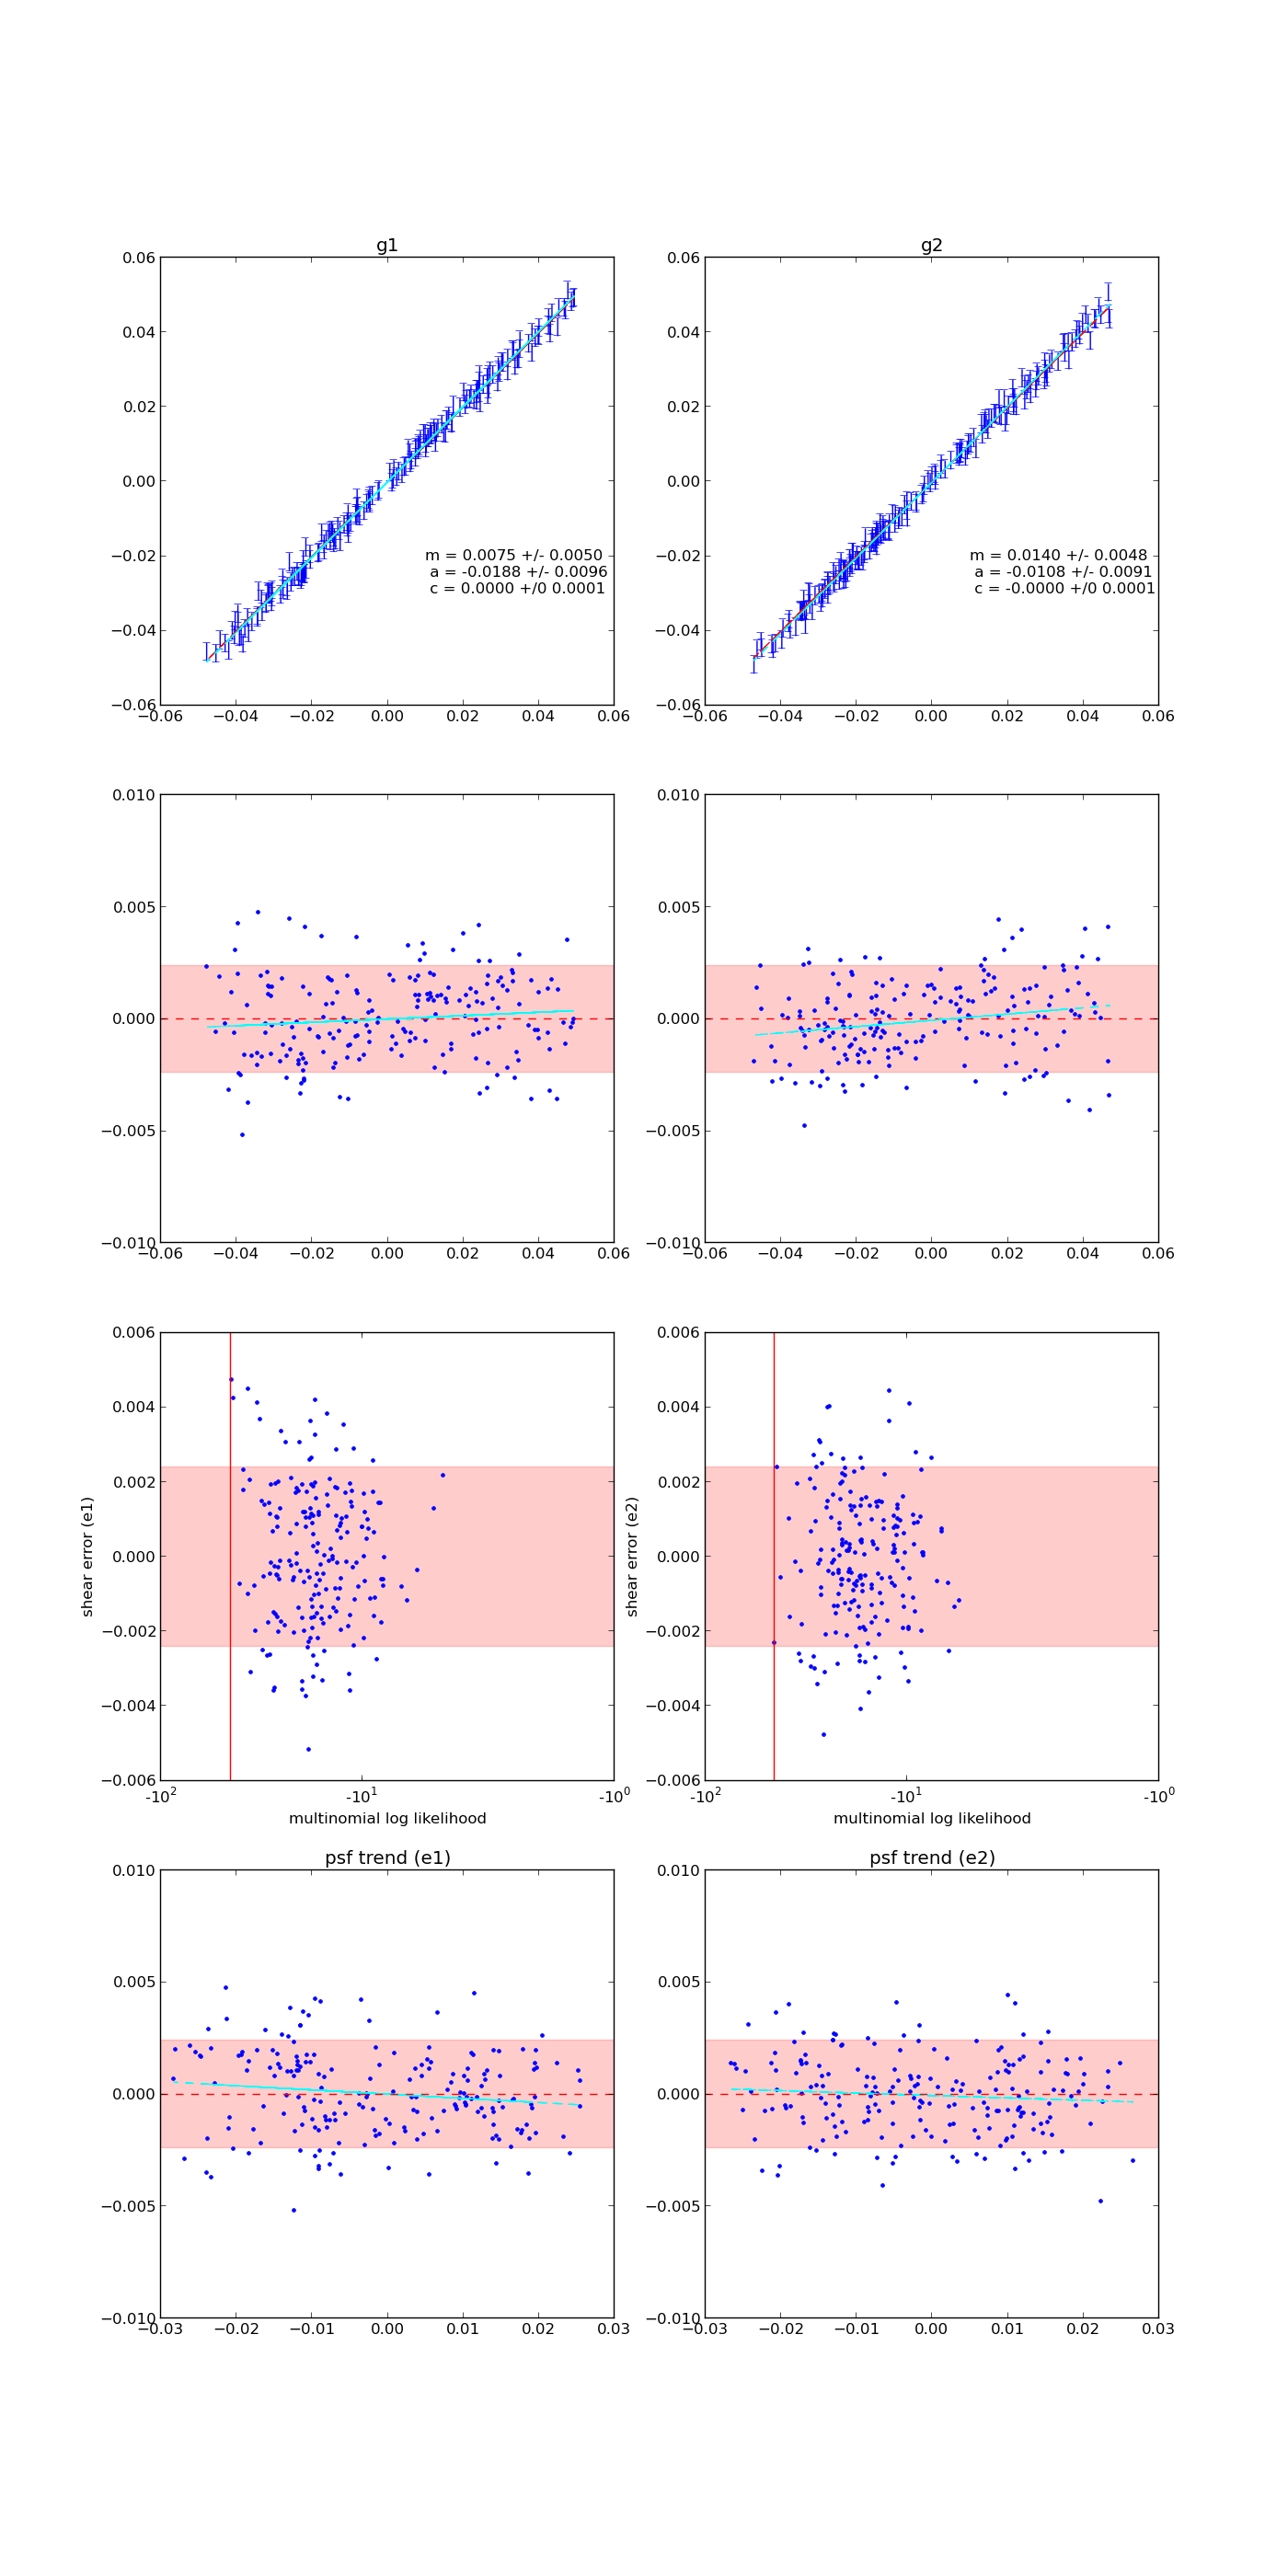
\includegraphics[width=0.31\linewidth]{./Plots/rgc-noaber-regauss-opt-shear_plots.png}
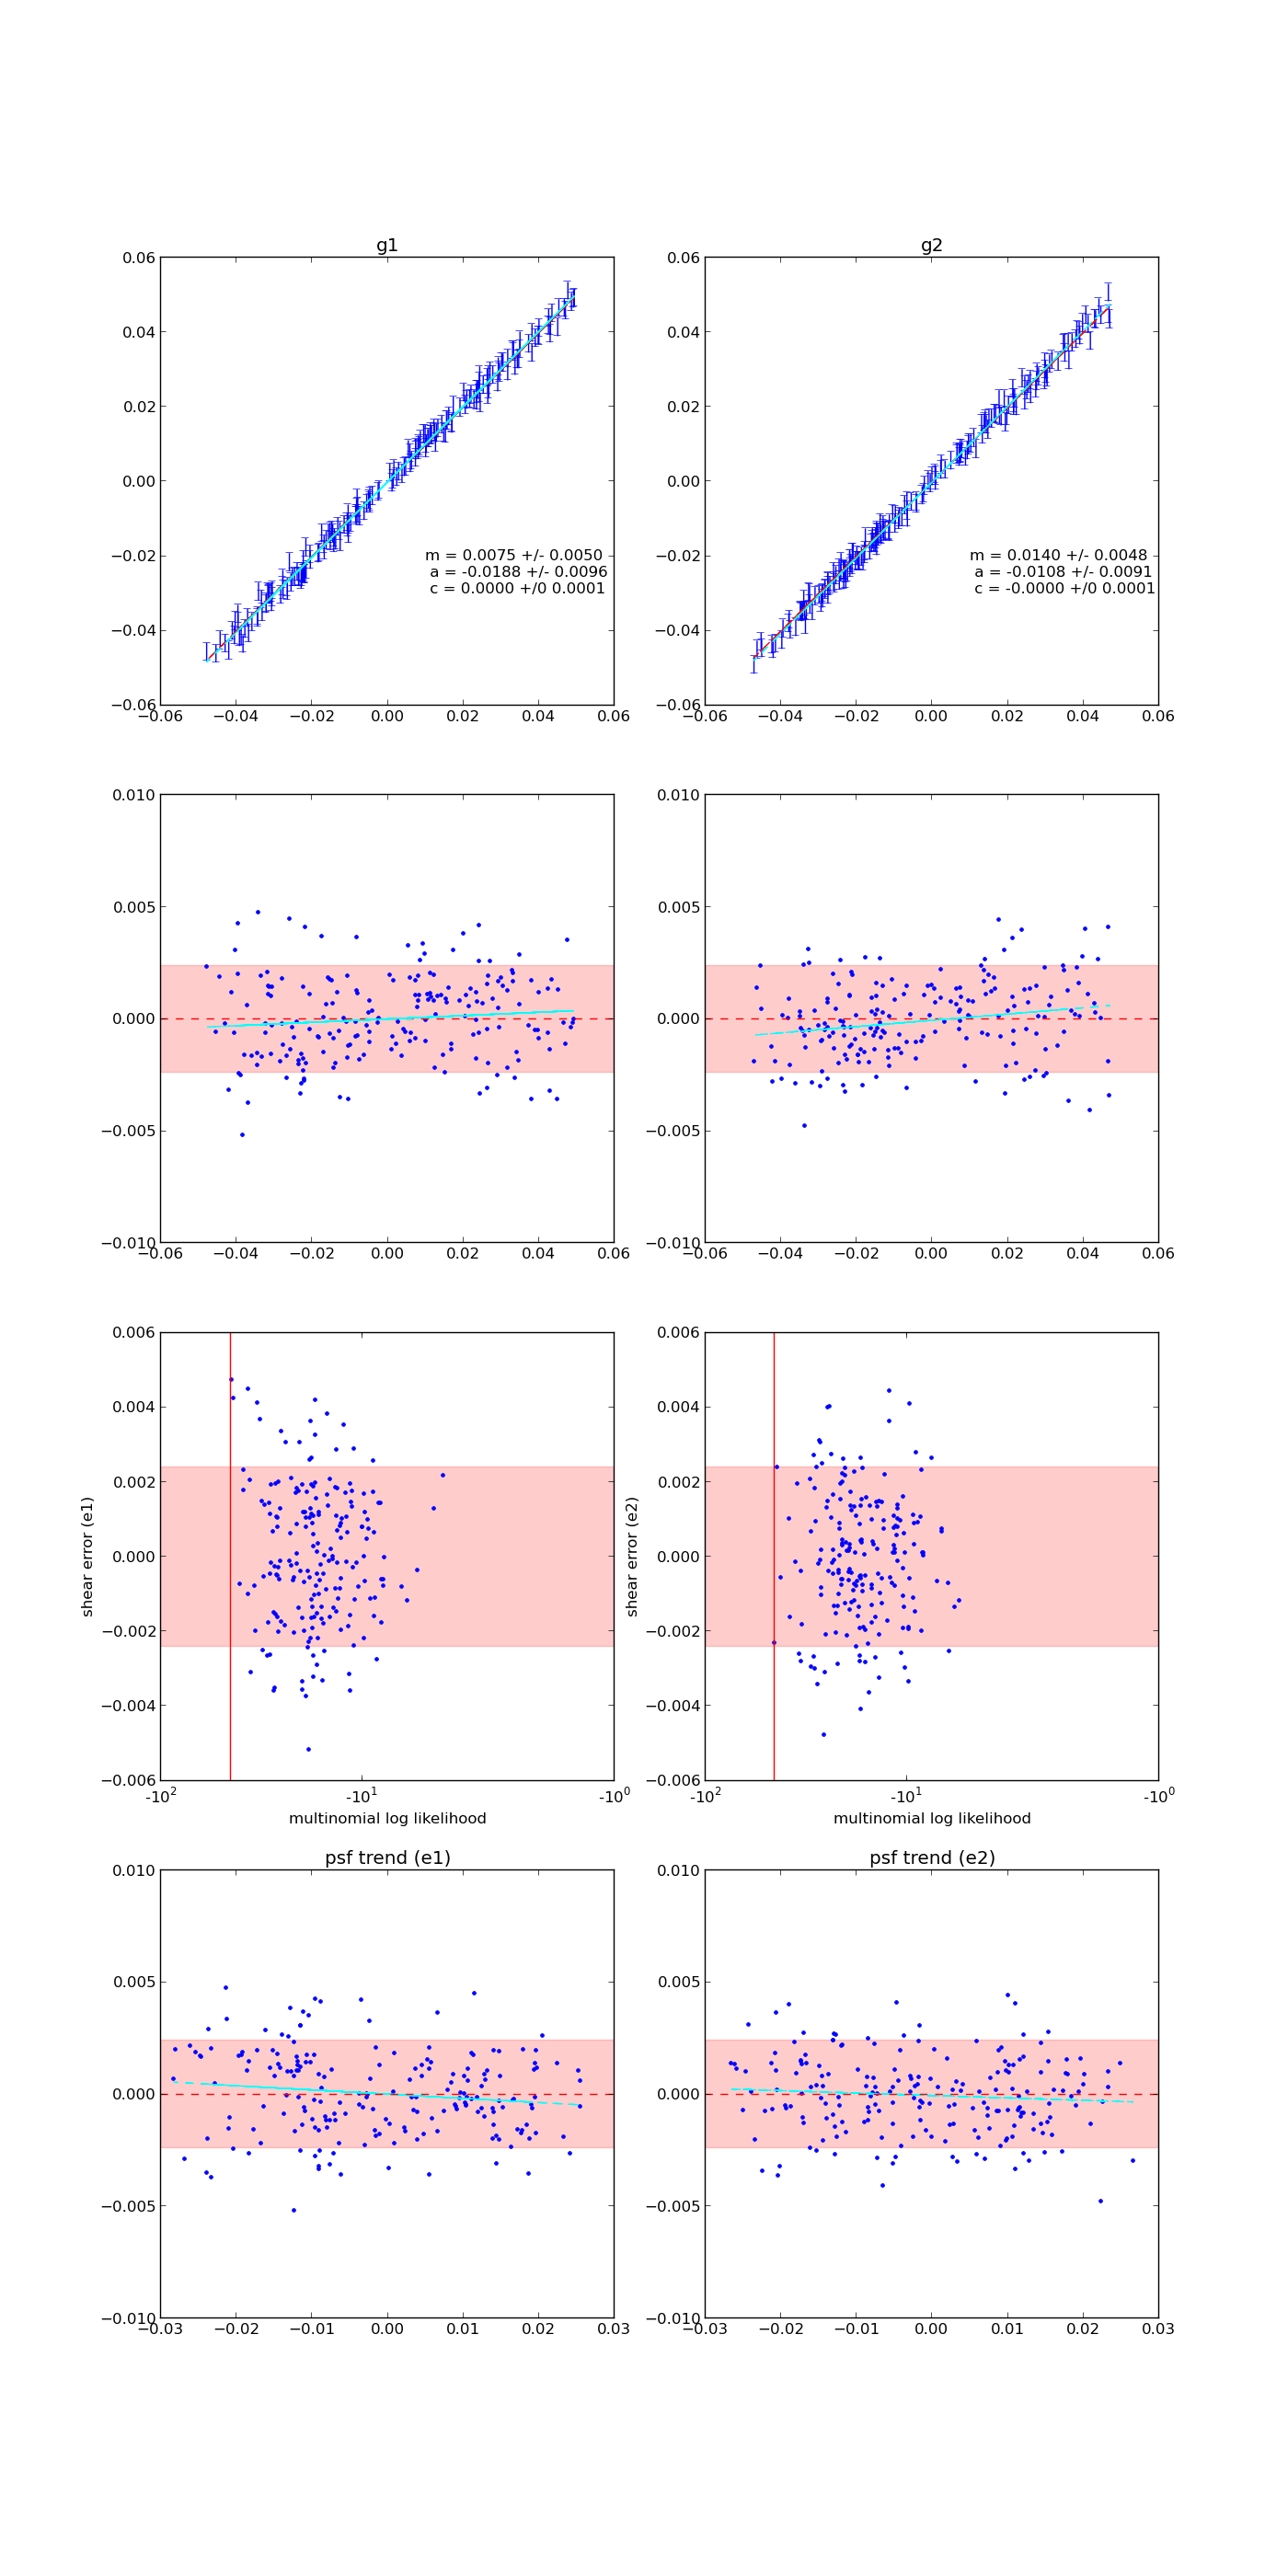
\includegraphics[width=0.31\linewidth]{./Plots/rgc-noaber-regauss-opt-shear_plots.png}
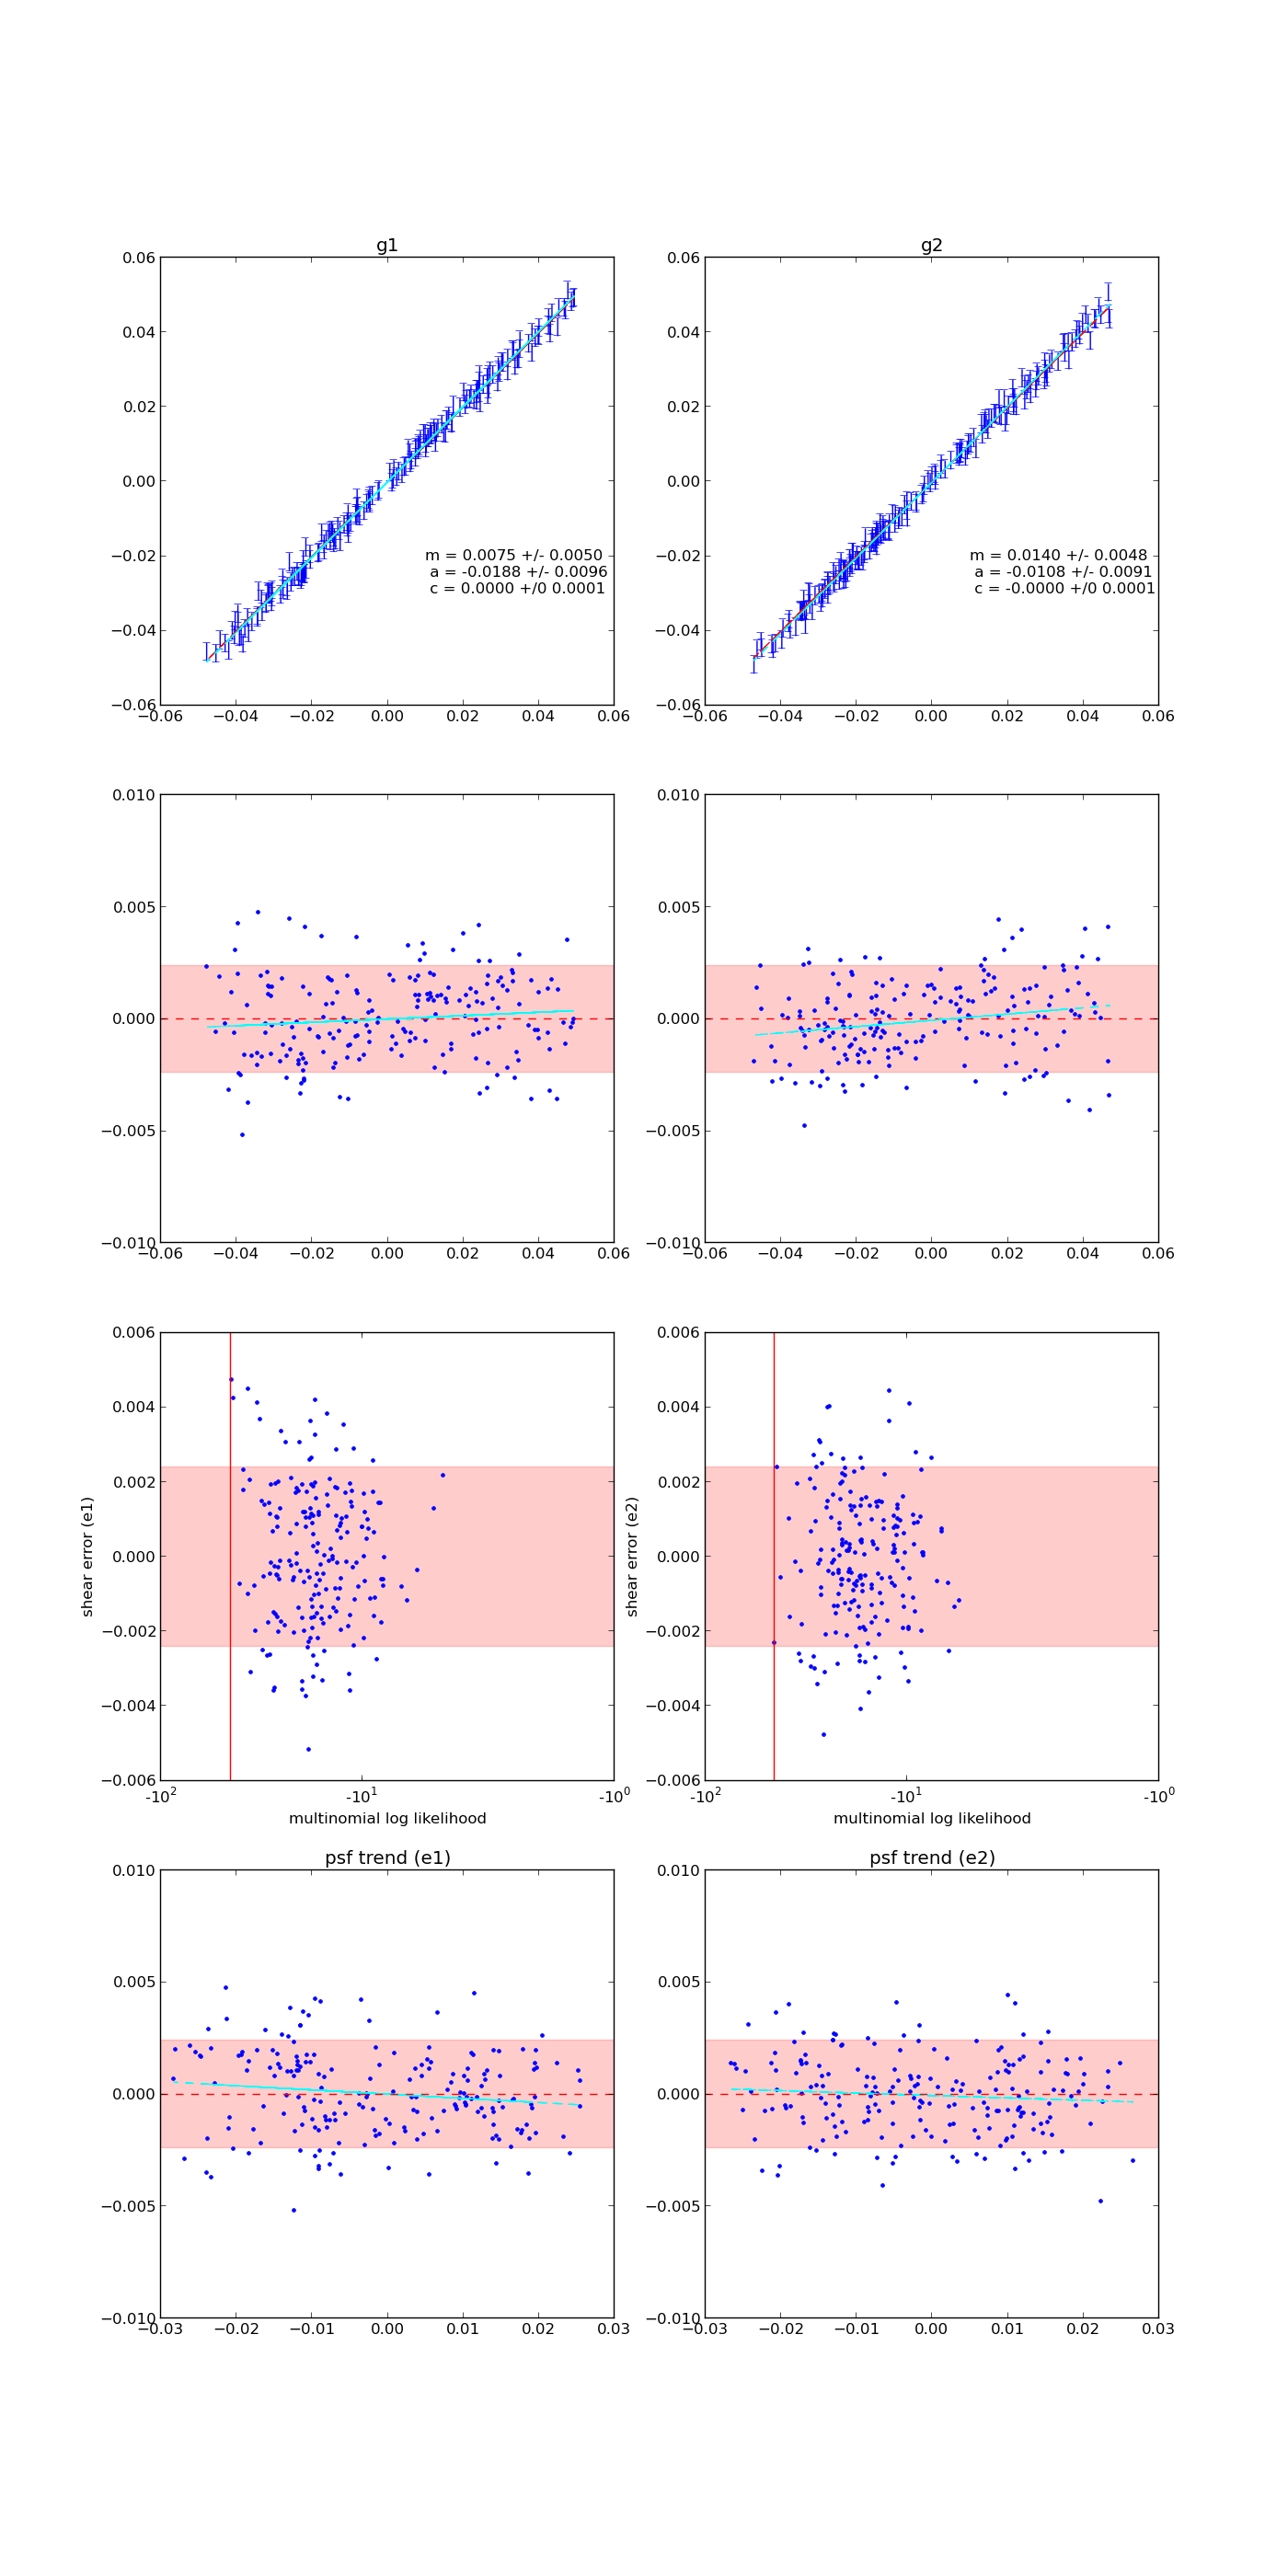
\includegraphics[width=0.31\linewidth]{./Plots/rgc-noaber-regauss-opt-shear_plots.png}
\caption{Results of metacalibration for regauss on RGC with no aberrations. From {\bf right} to {\bf left}: regauss, ksb, moments. Note that we do not have these results for ksb and moments yet.}
\end{figure*}



\begin{figure*}
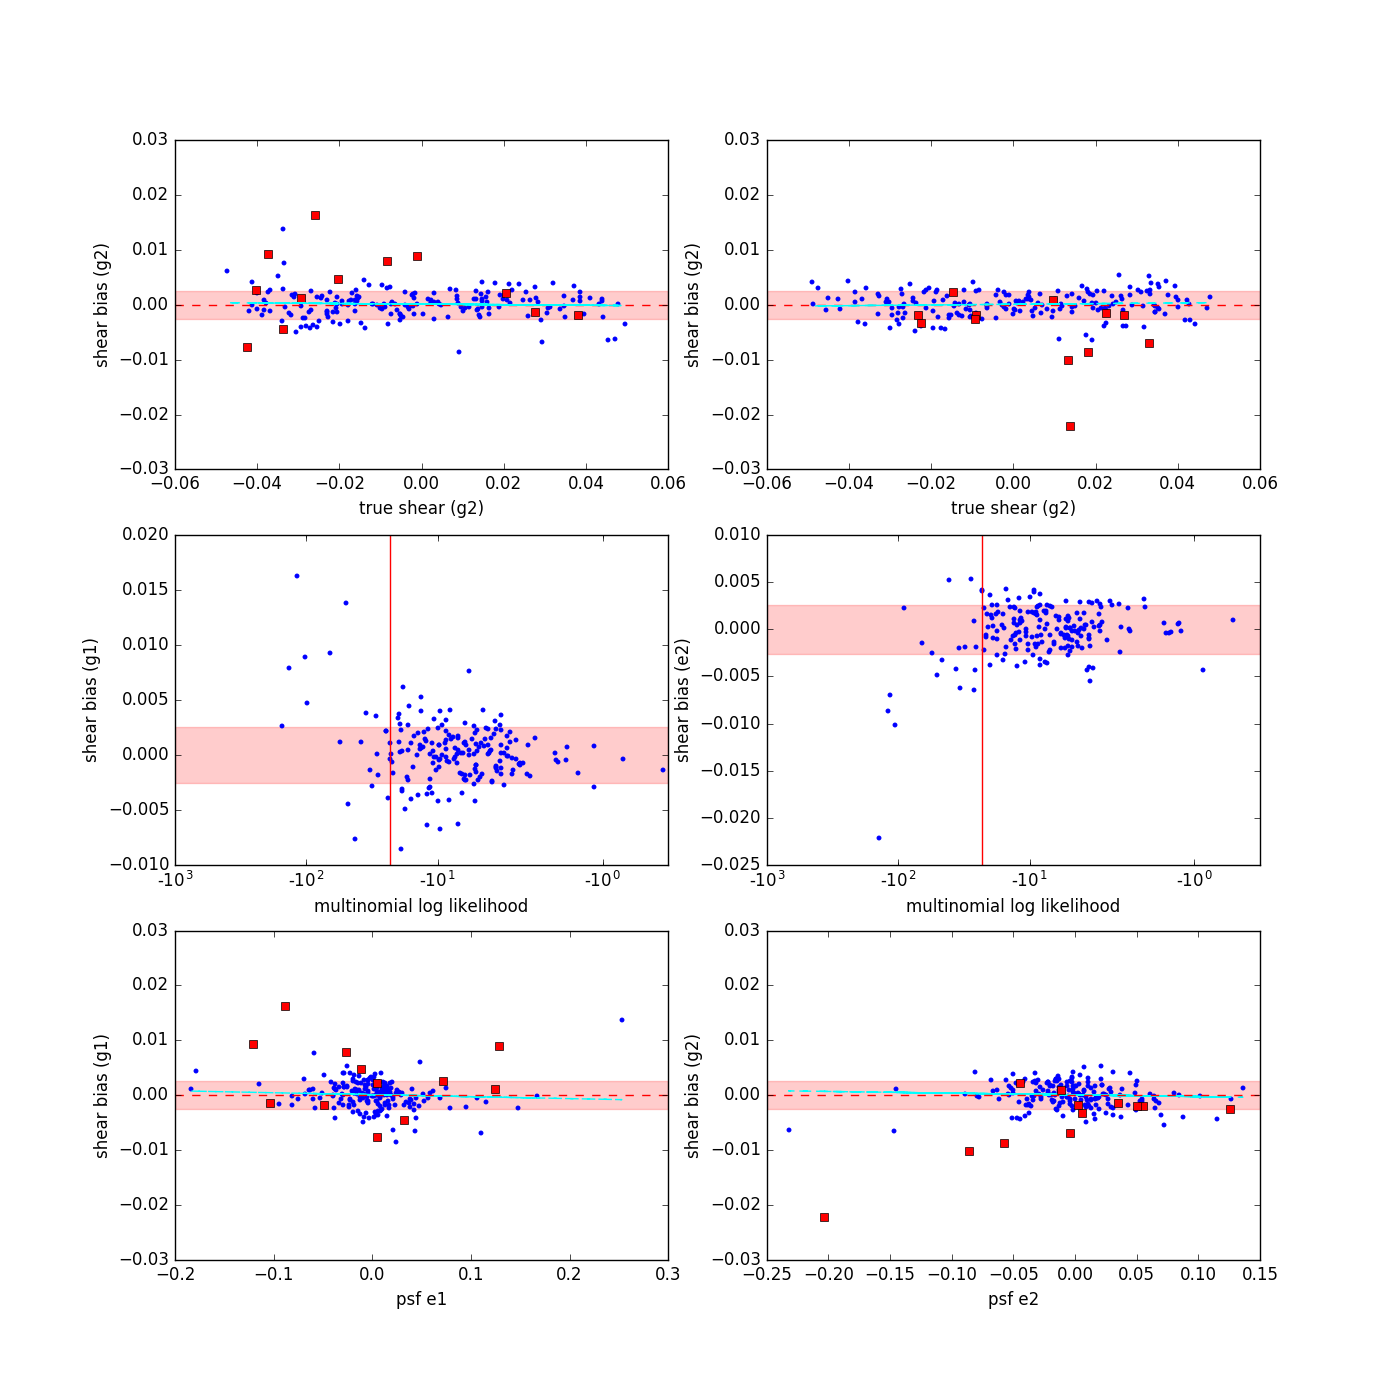
\includegraphics[width=0.31\linewidth]{./Plots/rgc-regauss-opt-shear_plots.png}
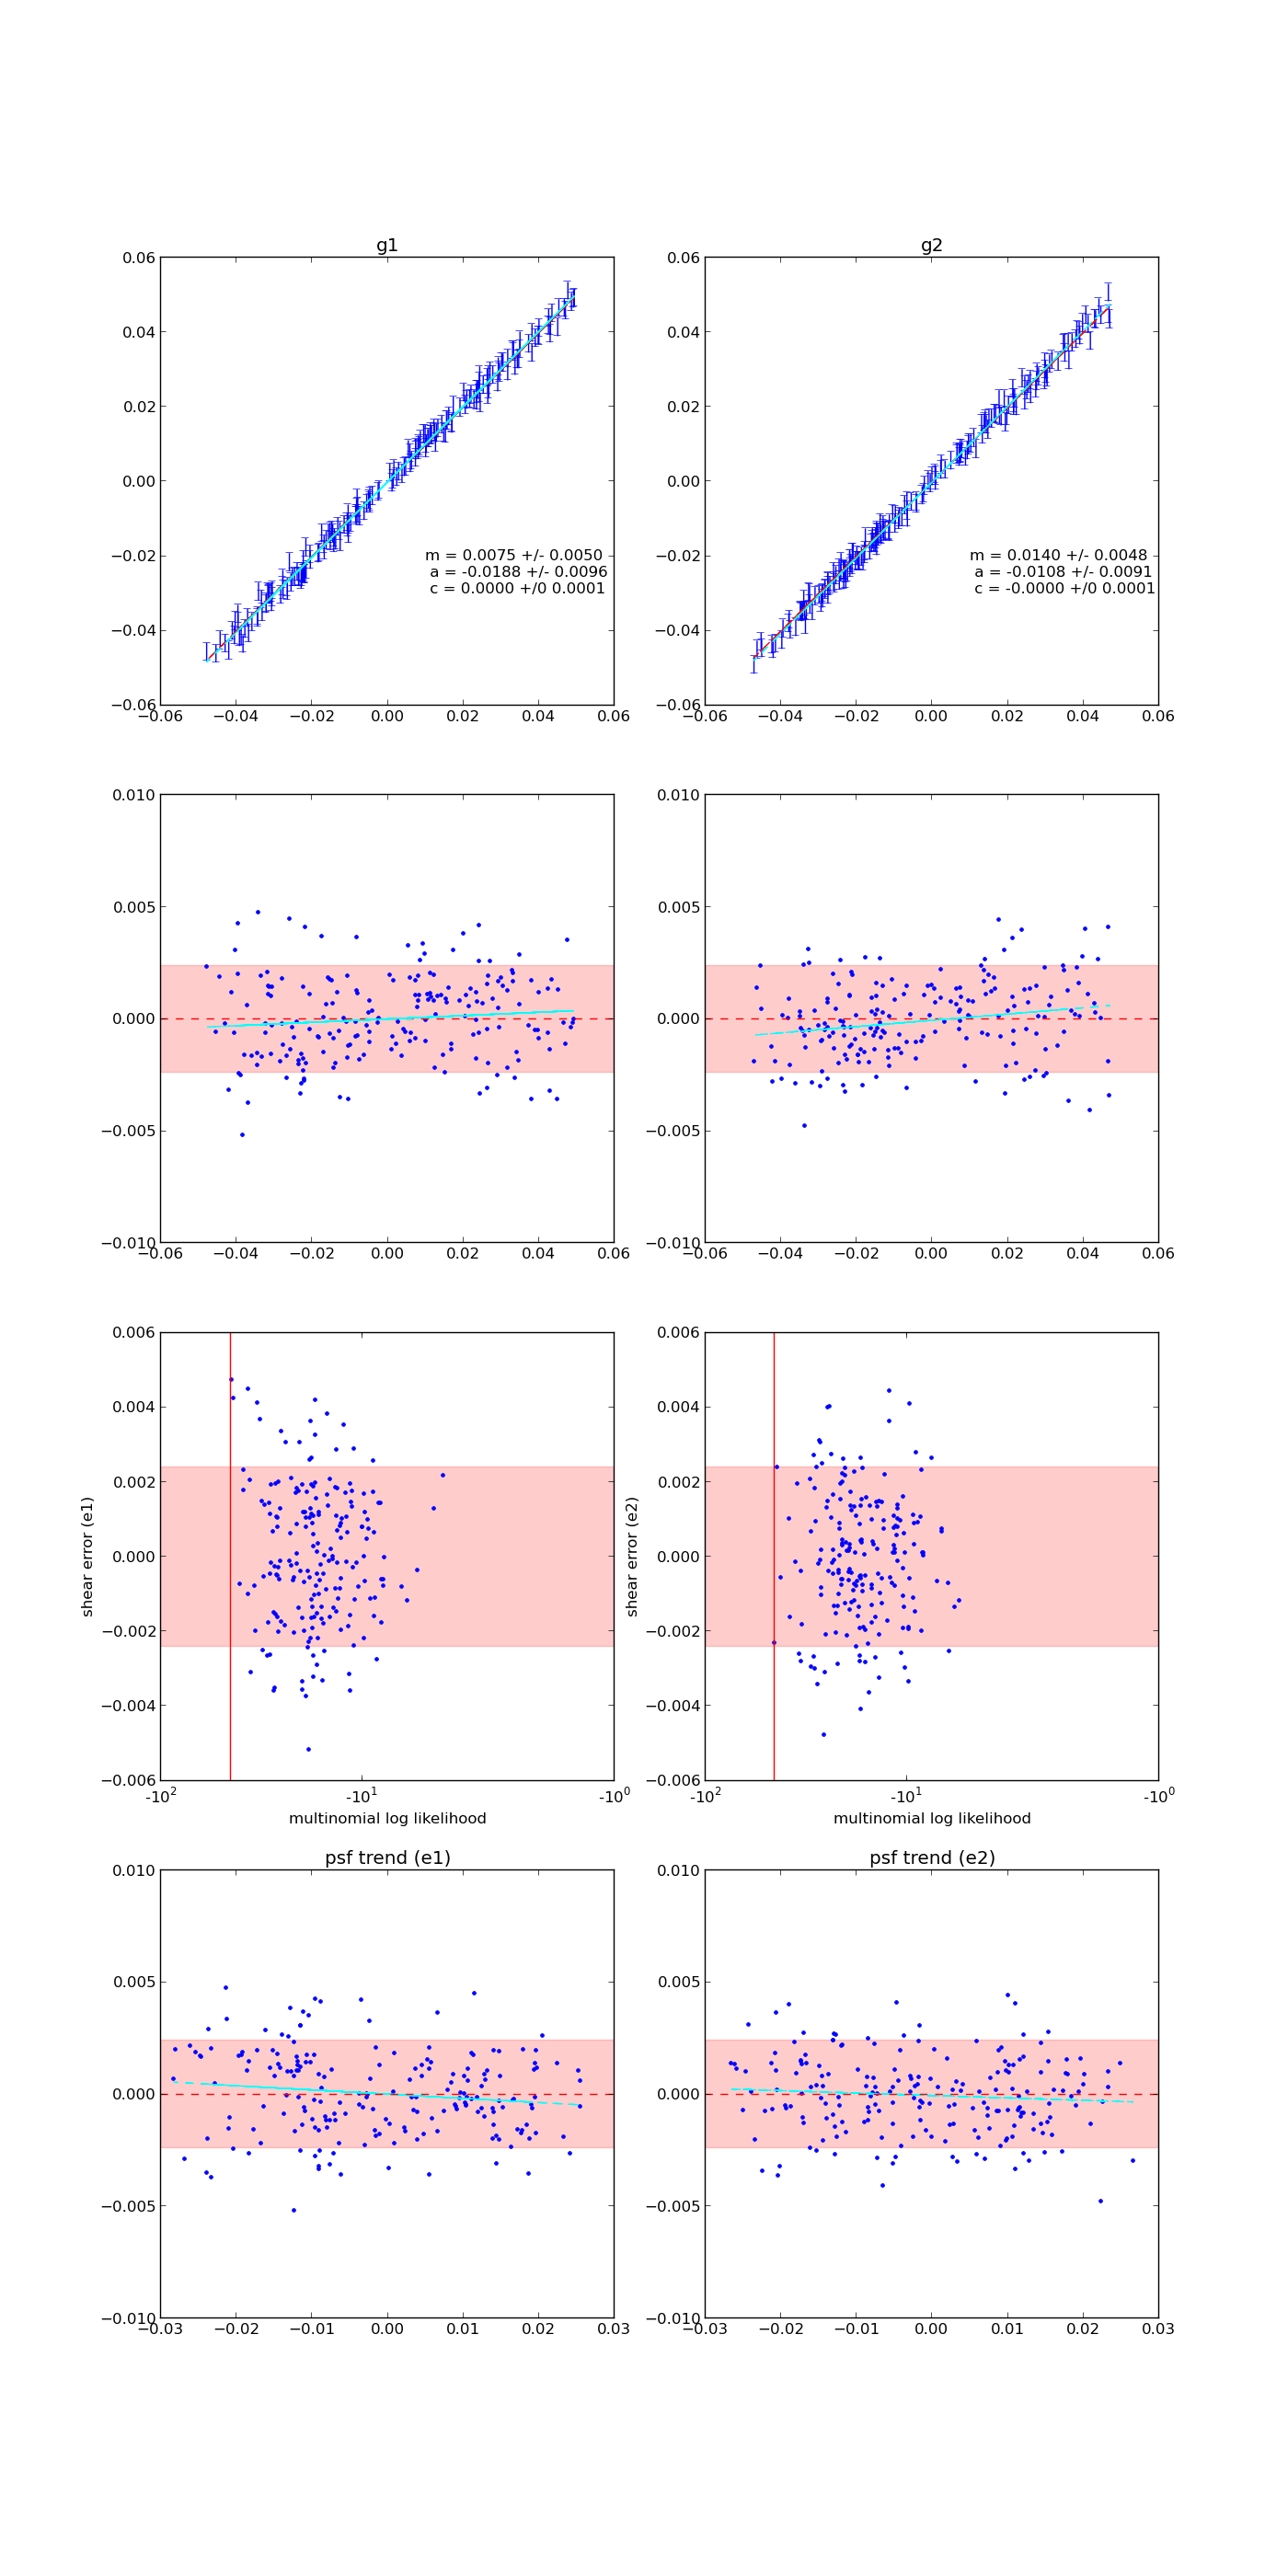
\includegraphics[width=0.31\linewidth]{./Plots/rgc-noaber-regauss-opt-shear_plots.png}
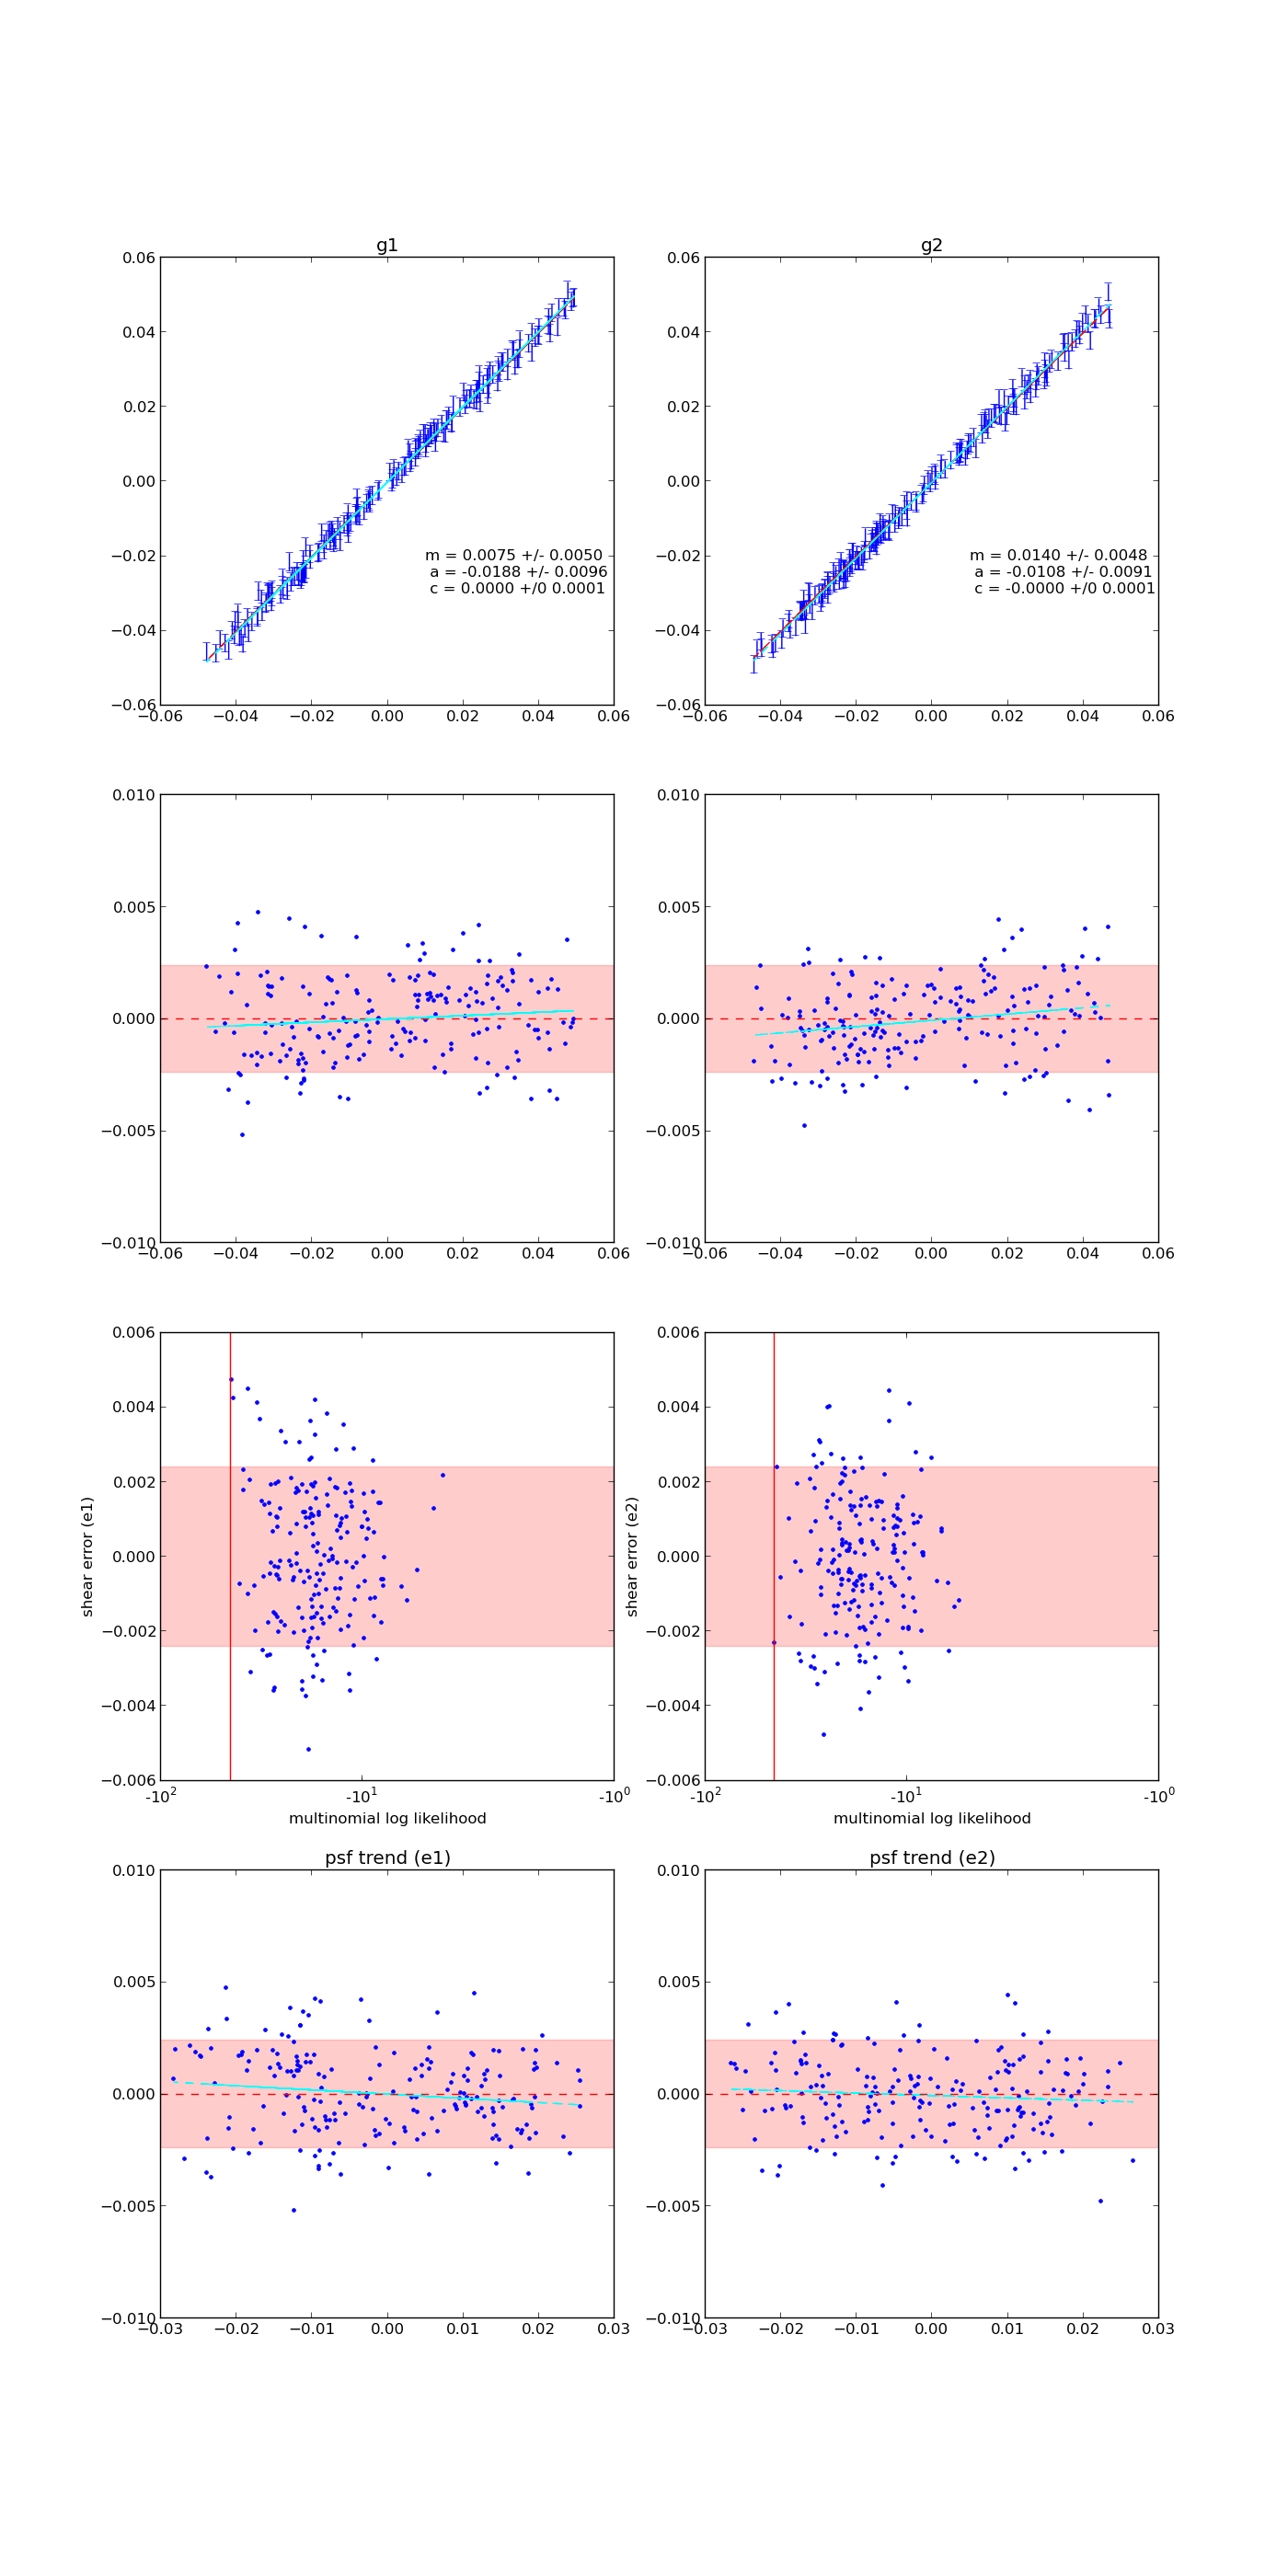
\includegraphics[width=0.31\linewidth]{./Plots/rgc-noaber-regauss-opt-shear_plots.png}
\caption{Results of metacalibration for regauss on RGC with aberrations. From {\bf right} to {\bf left}: regauss, ksb, moments. Note that we do not have these results for ksb and moments yet.}
\end{figure*}


\begin{figure*}
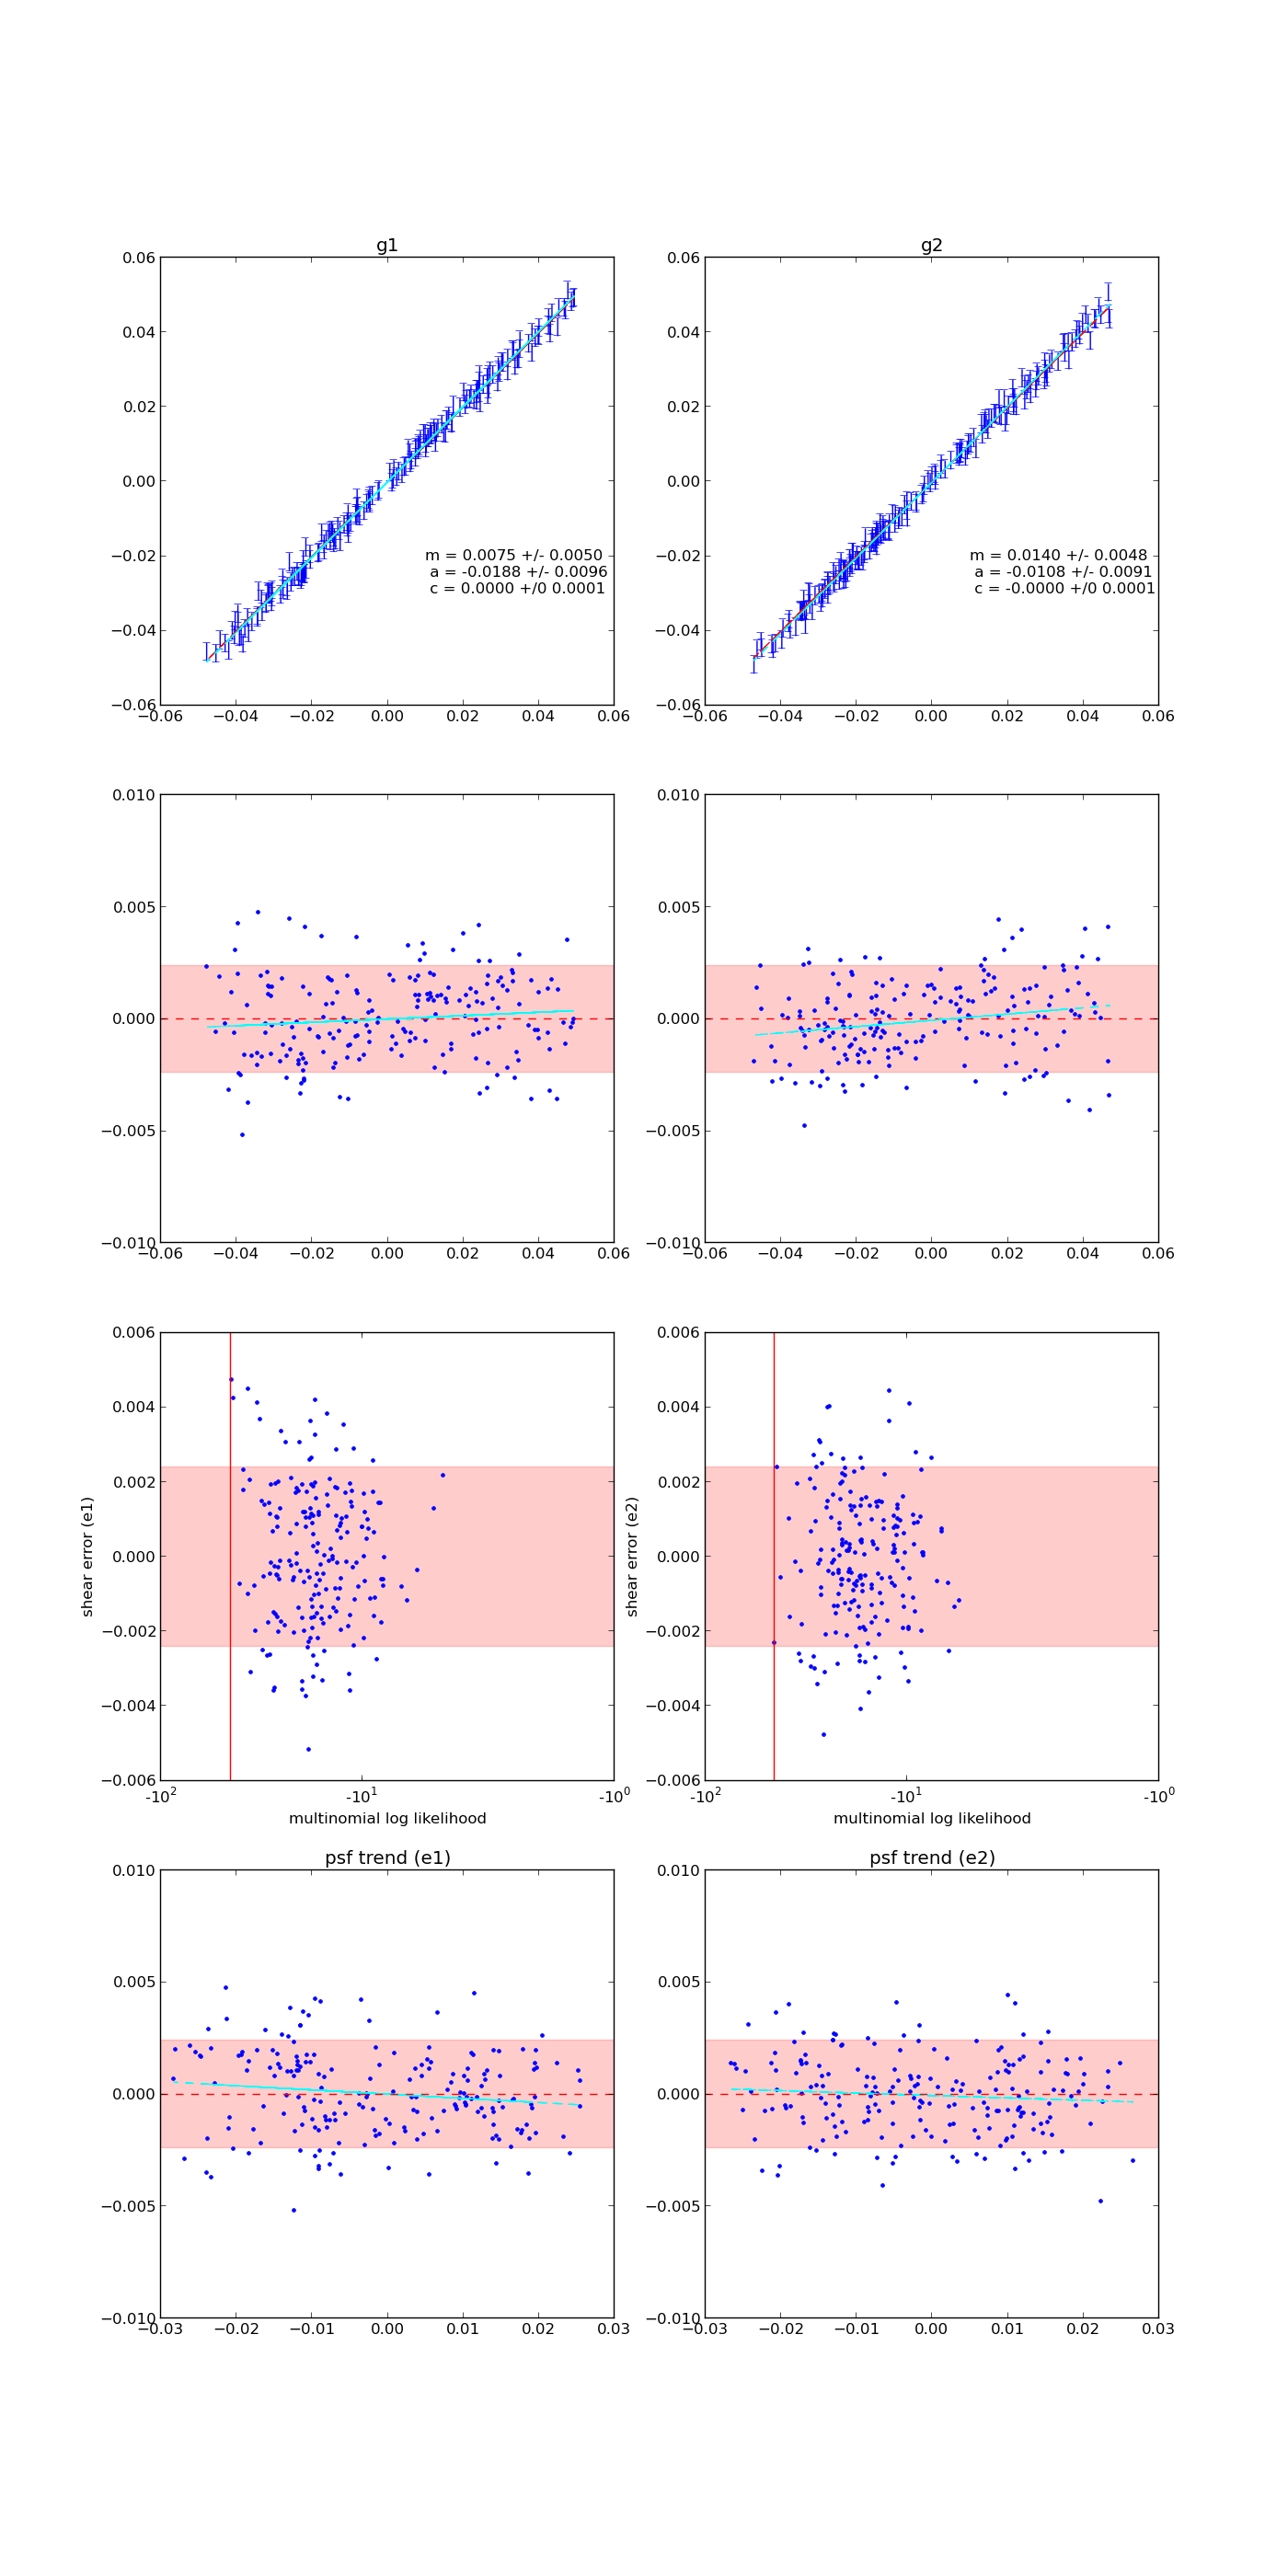
\includegraphics[width=0.3\linewidth]{./Plots/rgc-noaber-regauss-opt-shear_plots.png}
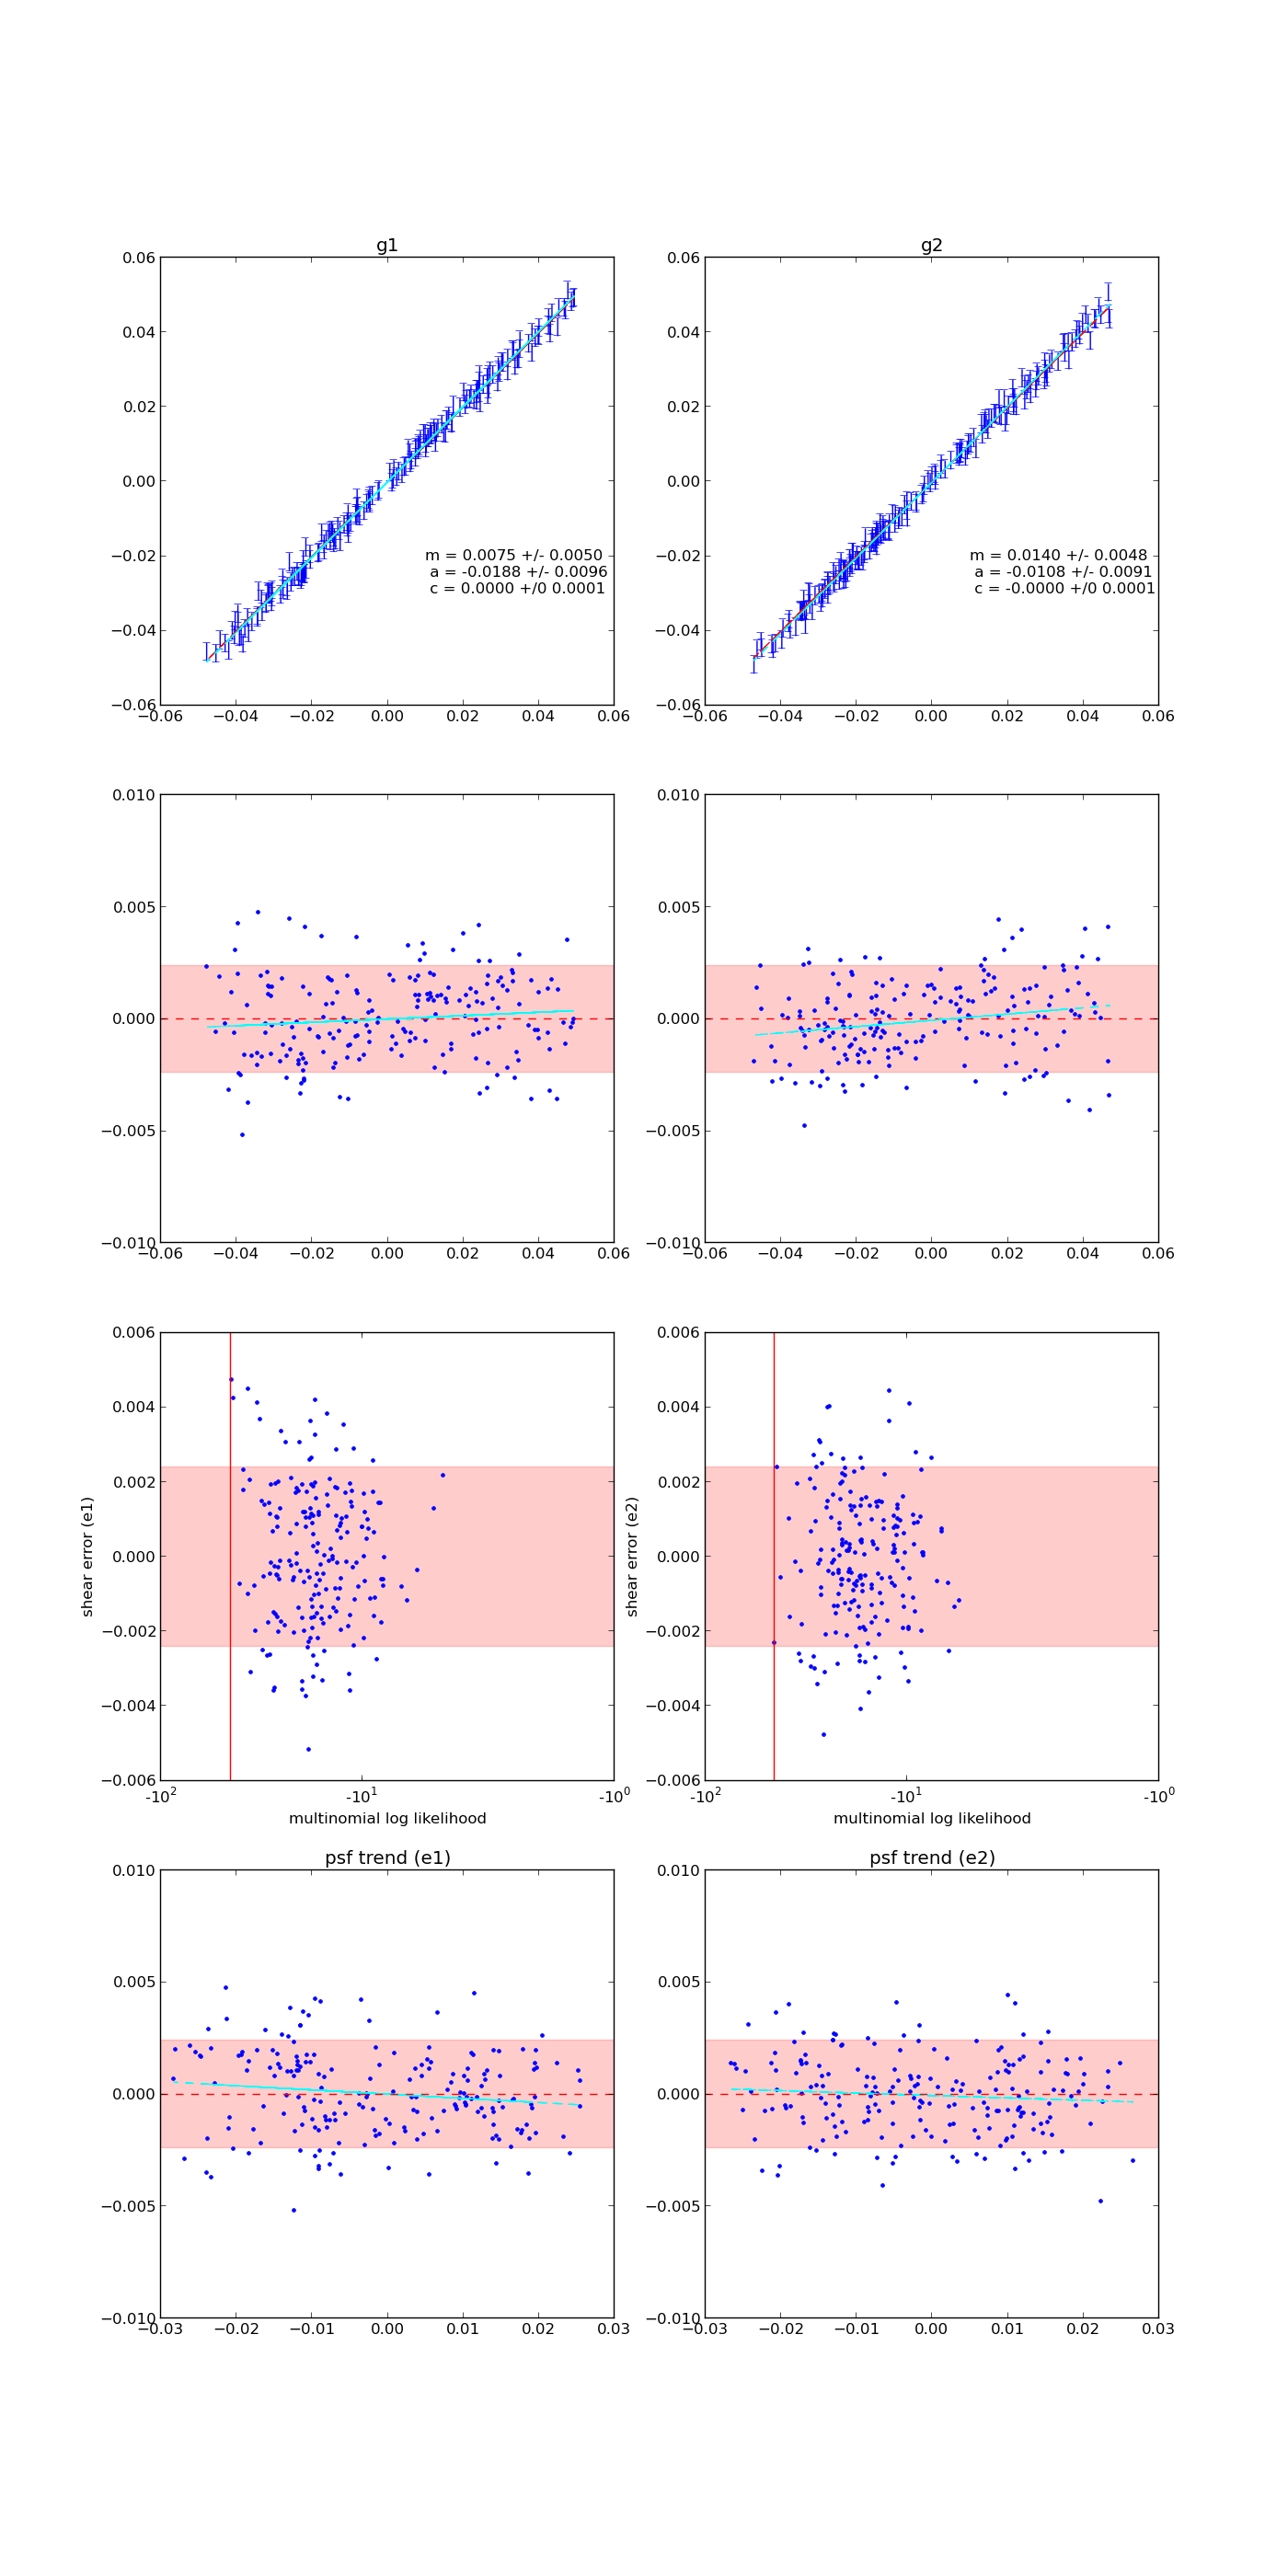
\includegraphics[width=0.3\linewidth]{./Plots/rgc-noaber-regauss-opt-shear_plots.png}
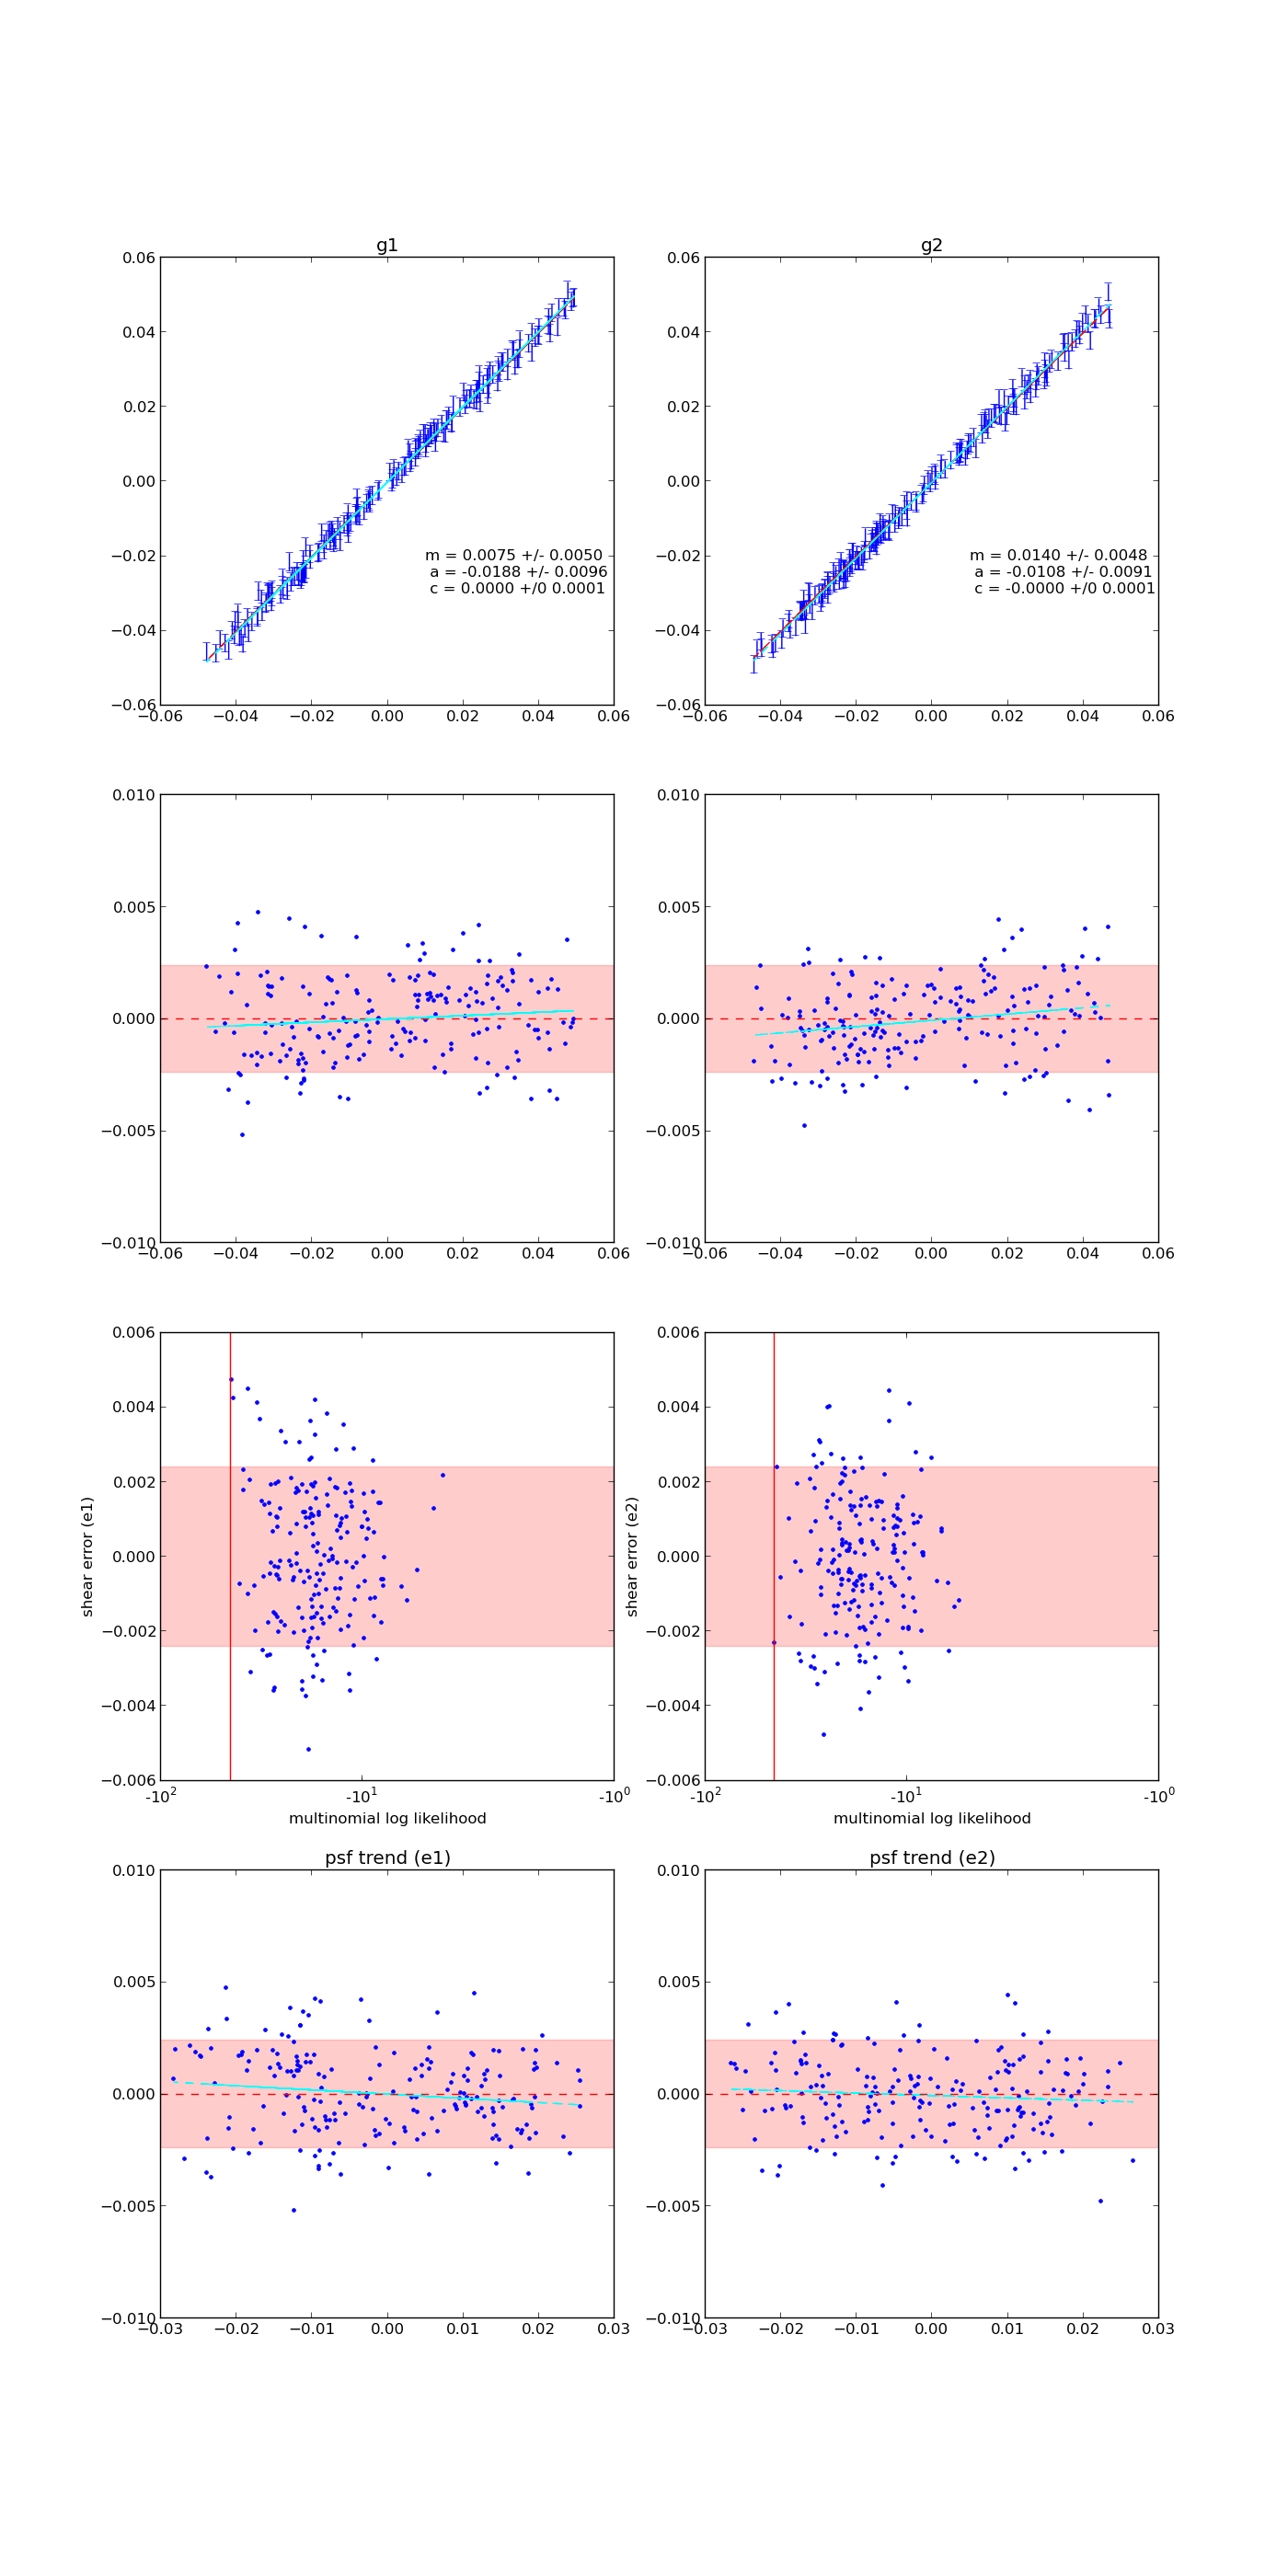
\includegraphics[width=0.3\linewidth]{./Plots/rgc-noaber-regauss-opt-shear_plots.png}
\caption{Results of metacalibration for regauss on RGC with large amplitude but small disperion aberrations. From {\bf right} to {\bf left}: regauss, ksb, moments. Note that we do not have these results for any method yet.}
\end{figure*}

\section{Results}
\towrite{Outline overall results, i.e., {\it veni, vidi, vici}}
\toplotemh{Table of Meta-Calibrated shear and psf calibration biases.}
\toplotrm{Something along the lines of: Great3-style plot showing before/after performance in some
  projection of m/c/a for regauss/ksb/possibly moments. Something that can easily be compared with
  one or more figures in the Great3 results paper.  Something like figure 17 with same axes and scaling.}


\section{Applicability to Real Data}
\towriteemh{Comment on effects that this method may deal with, which we haven’t tested (selection
  biases, other systematics detrending - lack of PSF knowledge?)}
\towriteemh{Comment on what measurements this can be straightforwardly applied to (mass mapping, g-g lensing) and what needs further thought (shear-shear) prior to deployment}
\towriteemh{Comment on effects that this method may or may not play well with -- blending, detector effects, nonlinearity, star-galaxy confusion}
\towriteemh{Comment on noise symmetrization -- we tried this, we don't understand why it didn't work as anticipated, but it doesn't seem to be important at this level of precision.}
\towriteemh{Put computational and implementation difficulty (for a realistic survey pipeline) in
  context. Is this substantially harder than making loads of independent sims? What are the
  prospects for further optimization, or other shortcuts? (silly things like 1-sided derivatives,
  but maybe there are others?)}




\section{Conclusions}
\towrite{Put performance measures from previous sections in context. How do these results compare
  with the state of the art? Will this be good enough for DES, Kids, LSST?, SuMiRE?}

\section*{Acknowledgments}

\towrite{Thanks to various people. Funding.}

\towrite{Some cleanup in references is needed.}

\bibliographystyle{apj}
\bibliography{bibliography}


\end{document}
